\documentclass[letterpaper,journal]{IEEEtran}

\usepackage{amsmath,amsfonts,amssymb}
\usepackage{bm}

\usepackage{algorithmic}
\usepackage{algorithm}

\usepackage{array}
\usepackage{booktabs}

\usepackage[caption=false,font=normalsize,
labelfont=sf,textfont=sf]{subfig}

\usepackage{textcomp}
\usepackage{stfloats}

\usepackage{url}
\usepackage{verbatim}

\usepackage{graphicx}
\usepackage{adjustbox}

\usepackage{cite}
\usepackage{balance}

\graphicspath{{fig3/}}

\hyphenation{
re-con-fig-ur-able
po-lar-i-met-ric
sub-car-ri-er
syn-chro-ni-za-tion
Cra-mer-Rao
}

\newtheorem{proposition}{Proposition}
\newtheorem{lemma}{Lemma}
\newtheorem{theorem}{Theorem}
\newtheorem{corollary}{Corollary}
\newtheorem{assumption}{Assumption}
\newtheorem{remark}{Remark}

% ---------------- shorthand ----------------
\newcommand{\R}{\mathbb{R}}
\newcommand{\C}{\mathbb{C}}
\newcommand{\bp}{\mathbf{p}}
\newcommand{\bx}{\mathbf{x}}
\newcommand{\by}{\mathbf{y}}
\newcommand{\ba}{\mathbf{a}}
\newcommand{\bb}{\mathbf{b}}
\newcommand{\bc}{\mathbf{c}}
\newcommand{\bd}{\mathbf{d}}
\newcommand{\be}{\mathbf{e}}
\newcommand{\bh}{\mathbf{h}}
\newcommand{\bg}{\mathbf{g}}
\newcommand{\bv}{\mathbf{v}}
\newcommand{\bw}{\mathbf{w}}
\newcommand{\bn}{\mathbf{n}}
\newcommand{\br}{\mathbf{r}}
\newcommand{\bs}{\mathbf{s}}
\newcommand{\bt}{\mathbf{t}}
\newcommand{\bq}{\mathbf{q}}
\newcommand{\bz}{\mathbf{z}}
\newcommand{\bu}{\mathbf{u}}
\newcommand{\bA}{\mathbf{A}}
\newcommand{\bBm}{\mathbf{B}}
\newcommand{\bC}{\mathbf{C}}
\newcommand{\bD}{\mathbf{D}}
\newcommand{\bE}{\mathbf{E}}
\newcommand{\bF}{\mathbf{F}}
\newcommand{\bG}{\mathbf{G}}
\newcommand{\bH}{\mathbf{H}}
\newcommand{\bI}{\mathbf{I}}
\newcommand{\bJ}{\mathbf{J}}
\newcommand{\bK}{\mathbf{K}}
\newcommand{\bL}{\mathbf{L}}
\newcommand{\bM}{\mathbf{M}}
\newcommand{\bP}{\mathbf{P}}
\newcommand{\bQ}{\mathbf{Q}}
\newcommand{\bR}{\mathbf{R}}
\newcommand{\bS}{\mathbf{S}}
\newcommand{\bT}{\mathbf{T}}
\newcommand{\bU}{\mathbf{U}}
\newcommand{\bV}{\mathbf{V}}
\newcommand{\bX}{\mathbf{X}}
\newcommand{\bY}{\mathbf{Y}}
\newcommand{\bN}{\mathbf{N}}
\newcommand{\bW}{\mathbf{W}}
\newcommand{\bZ}{\mathbf{Z}}
\newcommand{\bTheta}{\boldsymbol{\Theta}}
\newcommand{\bPsi}{\boldsymbol{\Psi}}
\newcommand{\bOmega}{\boldsymbol{\Omega}}
\newcommand{\bSigma}{\boldsymbol{\Sigma}}
\newcommand{\bPi}{\boldsymbol{\Pi}}
\newcommand{\brho}{\boldsymbol{\rho}}
\newcommand{\bmu}{\boldsymbol{\mu}}
\newcommand{\bchi}{\boldsymbol{\chi}}
\newcommand{\bxi}{\boldsymbol{\xi}}
\newcommand{\bvt}{\boldsymbol{\vartheta}}
\newcommand{\balpha}{\boldsymbol{\alpha}}
\newcommand{\Real}{\operatorname{Re}}
\newcommand{\Imag}{\operatorname{Im}}
\newcommand{\rank}{\operatorname{rank}}
\newcommand{\tr}{\operatorname{tr}}
\newcommand{\diag}{\operatorname{diag}}
\newcommand{\blkdiag}{\operatorname{blkdiag}}
\newcommand{\clip}{\operatorname{clip}}
\newcommand{\median}{\operatorname{median}}
\newcommand{\coll}{\operatorname{col}}
\newcommand{\cond}{\operatorname{cond}}
\newcommand{\unvec}{\operatorname{unvec}}

% Float separation: tightened from the IEEEtran defaults so that eight floats
% do not accumulate most of a column of white space.
\setlength{\textfloatsep}{13pt plus 2pt minus 5pt}
\setlength{\dblfloatsep}{13pt plus 2pt minus 5pt}
\setlength{\dbltextfloatsep}{13pt plus 2pt minus 5pt}
\setlength{\floatsep}{11pt plus 2pt minus 5pt}
\begin{document}

\title{Maxwell--Jones Vector-Sensor Localization and Synchronization for
Distributed Near-Field RIS-Aided OFDM}

\author{Qingshan Gong,~\IEEEmembership{Member,~IEEE}}

\markboth{IEEE Transactions on Wireless Communications,~Vol.~XX, No.~XX, 2026}%
{Gong: Maxwell--Jones Vector-Sensor Localization and Synchronization}

\maketitle

\begin{abstract}
We address near-field localization and clock synchronization by jointly estimating
a single-antenna user's 3-D position and common clock offset from its
orthogonal frequency-division multiplexing (OFDM) uplink, which reaches
one electromagnetic vector-sensor (EVS) array only through distributed
near-field reconfigurable intelligent surface (RIS) panels. Jones-domain path
coefficients and cascade-to-panel association are unknown. A
per-panel space--frequency/Maxwell--Jones factorization shows that
receiver-component selection rescales local information but can eliminate
panel separability. Calibration fixes a Maxwell receive subspace independent
of position and clock. In the reference scene, projection before acquisition
reduces $96$ receive dimensions to $6$. Under the matched white-Gaussian
model, the profiled maximizer and free-Jones equivalent Fisher information
matrix are unchanged, as is the resulting Cram\'er--Rao bound when finite.
In Jones variable projection, the profiled Gram matrix is clock-invariant. At fixed
position, the conditional clock profile is a trigonometric polynomial with a
deterministic optimality-gap certificate; the outer search is 3-D. At a
signal-to-noise ratio of $-10$~dB in the
matched center-frequency reference scene, the estimator has a $0.32$-mm
median position error and position and clock catastrophic rates of $0.42\%$
and $0.31\%$, $6.0$- and $6.7$-fold lower than the closest in-model control.
\end{abstract}

\begin{IEEEkeywords}
Clock synchronization, Cram\'er--Rao bound, EVS, near-field localization,
OFDM, RIS, variable projection.
\end{IEEEkeywords}


\section{Introduction}
\label{sec:introduction}

\IEEEPARstart{I}{n} the near field of an electrically large reconfigurable
intelligent surface (RIS) panel, the phase across the aperture depends on
the direction and propagation range of the user equipment (UE) relative to
the panel~\cite{wymeersch2020risloc,cui2023nearfield}. A surveyed panel can use
this variation to constrain the UE position in three
dimensions~\cite{elzanaty2021bounds,zhu2026mixed}. With the direct link
blocked, the base station (BS) observes cascades through
distributed panels~\cite{xia2026nlos}. Each cascade combines geometric delay
with the same UE clock offset; the passive panels supply no independent
timing reference.

Distributed-RIS localization combines geometric constraints from multiple
panel paths~\cite{ma2023distributed,liu2025multiris,zhu2025hybrid}, and several
formulations jointly estimate an unknown clock
offset~\cite{fascista2022rissync,gong2024async,peng2025sdp,yan2025ris,fadakar2024multiris}.
Near-field estimators retain spherical-wave phase across electrically large
apertures~\cite{liu2025corr}. Multilinear methods factor the training
tensor~\cite{lin2021tensor,cao2025tensorris}. With all cascades observed at
one array, the factors returned by an algebraic front end still need to be
assigned to surveyed panels before the geometric fit. Sparse and
variational methods estimate parameters on a discretized
manifold~\cite{li2024vbi}; polar or beam-split codebooks search direction and
range~\cite{cui2022channel,yang2024nfris,zheng2025wideband}. Resolving finer
aperture-scale detail with a fixed grid increases the dictionary or search
density.

Dual-polarized RISs use polarization for beamforming
gain~\cite{han2022dual,zheng2025dualpol}, whereas an electromagnetic vector
sensor (EVS) measures co-located electric and magnetic fields to estimate the
incident polarization together with its
direction~\cite{nehorai1994vector,khan2020sixcomponent,lan2026vecpol}.
RIS-aided EVS radar extends this processing to joint departure-angle,
arrival-angle and polarization estimation~\cite{yu2026emvsris}. Our previous
EVS estimator for orthogonal frequency-division multiplexing
(OFDM)~\cite{gong2026aimdf} treats a direct multipath channel. The distributed
cascades add panel association and a common clock to the geometric fit.

First, distributed-RIS methods typically resolve cascade-to-panel association
before or during the joint
fit~\cite{ma2023distributed,liu2025multiris,fascista2022rissync}. All
cascades reach the same EVS array within one observation, and an algebraic
front end returns them unlabeled~\cite{lin2021tensor}. Panels with nearly
coincident delays then present similar space--frequency evidence, making
separability depend on the retained Maxwell structure of the receiver.
Second, full-EVS training produces six field components over $M_A$ sensors,
$N$ subcarriers and $T$ configurations; a general linear reduction need not
preserve the delay subspace, profiled likelihood or localization information.
Third, differencing cascaded OFDM delays removes the common clock but leaves
only $K-1$ differences for three coordinates and is underdetermined at $K=3$.
Retaining the absolute delays gives a nonconvex 4-D position--clock problem.
Variable projection~\cite{golub1973varpro} eliminates the linear nuisances but
leaves position and clock coupled. The semidefinite method
of~\cite{peng2025sdp} uses a timing model with a linear lifting, which the
cascaded OFDM likelihood does not admit.

The sensing block of the $k$th RIS panel factorizes as
\begin{equation}
	\bA_k(\bchi)=
	\underbrace{\bc_k(\bchi)}_{\text{space--frequency geometry}}
	\otimes
	\underbrace{\bTheta_k^{({\rm mode})}}_{\text{calibrated Maxwell--Jones}},
	\label{eq:premise}
\end{equation}
where $\bchi=[\bp^{\mathsf T},\Delta t]^{\mathsf T}$ collects the unknown
position and clock, $\bc_k$ depends on both, and
$\bTheta_k^{({\rm mode})}$---two columns for the polarization state, one row
per retained field component---is fixed by the calibrated RIS-to-BS geometry
and the selected receiver mode.

\textbf{C1. Receiver-mode information and panel separability.} Component
selection rescales a panel's free-Jones equivalent Fisher information matrix
(EFIM), with Jones coefficients treated as unknown nuisances, by the retained
polarization energy without
changing its eigenvectors. Panel separability instead depends on a residual
in the retained Maxwell receive subspace; this residual can vanish with no
more than two field components even when the local EFIM remains finite
(Theorem~\ref{thm:split}; Figs.~\ref{fig:c1_receiver}
and~\ref{fig:c1_separability}).

\textbf{C2. Calibrated sufficient compression.} Calibration fixes the Maxwell
receive subspace independently of $\bchi$. In the reference scene, projecting
onto it reduces the receive dimension from $96$ to $6$. For the matched
white-Gaussian model, the projected data preserve the profiled maximizer and
free-Jones EFIM exactly. They are sufficient when the variance is known;
with unknown variance, sufficiency also requires the discarded energy.
In the finite-sample test, removing
the other $90$ directions improves delay-subspace acquisition
(Theorem~\ref{thm:compress}; Table~\ref{tab:c2_ladder}).

\textbf{C3. Certified common-clock profiling.} Over equispaced tones, the
clock acts through a finite diagonal phase orbit and leaves the profiled Gram
matrix invariant. After eliminating the linear coefficients, its conditional
profile is a trigonometric polynomial with a deterministic optimality-gap
certificate. Eliminating the clock leaves a unit-invariant 3-D outer search
(Theorem~\ref{thm:clock}; Table~\ref{tab:c3_control}).

Gaussian sufficiency for a known signal subspace and elimination of linear
parameters by variable projection are classical. Calibration fixes the
required subspace without knowing $\bchi$. The delay front end reuses the
asymmetric tensor folding of~\cite{gong2026aimdf}; this paper adds the
preceding sufficient compression and the following common-geometry fusion.

The C1 split applies to any array whose response factorizes into a
calibrated polarimetric block and a parameter-dependent geometric one. C3
extends to separable least-squares problems in which the nuisance follows an
equispaced finite Fourier phase orbit and the profiled Gram matrix is nuisance
invariant; under those conditions, the conditional profile remains a
trigonometric polynomial that can be maximized globally with a certificate.

Notation: bold symbols denote vectors and matrices; $(\cdot)^{\mathsf T}$,
$(\cdot)^{\mathsf H}$, $(\cdot)^{\ast}$ and $(\cdot)^{\dagger}$ are transpose,
Hermitian transpose, entrywise complex conjugation and pseudoinverse;
$\otimes$ and $\odot$ are Kronecker and
Hadamard products; for a generic matrix $\bX$, $\bP_{\bX}=\bX\bX^{\dagger}$
and $\bPi_{\bX}^{\perp}=\bI-\bP_{\bX}$ are the orthogonal projectors onto
$\coll(\bX)$ and $\coll(\bX)^{\perp}$; $\|\cdot\|_F$ is the Frobenius norm;
and unqualified vector and matrix norms are Euclidean and spectral,
respectively.

\section{Maxwell--Jones Cascaded Signal Model}
\label{sec:system_model}

The signal from a single-antenna UE reaches the BS only through $K$
distributed, arbitrarily oriented RIS panels; the line-of-sight (LoS) path is
blocked~\cite{fascista2022rissync,zhao2021timing}. Each panel is an
$M_{Rx}\times M_{Ry}$ planar array of $M_R=M_{Rx}M_{Ry}$ elements, and the BS
is an $M_A$-element EVS uniform linear array (ULA); the UE transmits pilots on
$N$ subcarriers spaced by $\Delta f$ (occupied bandwidth
$B_{\rm occ}=(N-1)\Delta f$) over $T$ known RIS phase configurations. The nonlinear parameters of interest are the
UE position $\bp$ and the clock offset $\Delta t$. Let $f_c$ denote the
carrier frequency and $c_0$ the speed of light; then $\lambda_c=c_0/f_c$
is the carrier wavelength.

\textbf{(A1)} The LoS path is blocked and each of the $K$
calibrated panels contributes one dominant cascade, so the model order is
known; Section~\ref{subsec:res_robustness} quantifies the effect of an
incorrect $K$. \textbf{(A2)} The BS and panel geometries are surveyed, and the
EVS Maxwell response and its per-component gains are
calibrated~\cite{bayraktar2024risloc}; Fig.~\ref{fig:boundaries}(a)--(b)
sweeps residual calibration error. \textbf{(A3)} Following the one-sided
near-field convention of~\cite{yang2024nfris,cui2022channel}, the UE--RIS hop
is modeled with an exact spherical-wave phase over a uniform-amplitude
aperture and the RIS--BS hop with a center-frequency plane wave;
Section~\ref{subsec:res_setup} verifies
$\max_k d_{{\rm UR},k}<R_{\rm FF}<\min_k d_{{\rm RB},k}$, where
$R_{\rm FF}=2D_{\rm ap}^2/\lambda_c$ is a panel's Fraunhofer distance and
$D_{\rm ap}$ its aperture diameter, the corner-to-corner span of the element
grid. \textbf{(A4)}
Spatial responses are evaluated at $f_c$ and the wideband dependence is
confined to the delay phase~\cite{wang2025wbnf}; the neglected
spatial-wideband phase reaches $\epsilon_{\rm sq}=0.102$~rad in the reference
scene. Section~\ref{subsec:res_setup} diagnoses
the resulting bias. \textbf{(A5)} The cyclic prefix covers the cascaded delay
spread and one common clock offset enters every delay; residual
carrier-frequency offset, phase noise and panel-dependent timing
offsets~\cite{zhao2021timing} lie outside the model. \textbf{(A6)} UE
position, clock, gains and Jones states are block-static over the $T$
configurations and the noise is white with unknown variance;
Section~\ref{subsec:res_robustness} reports the coherence budget.

The received signal is
\begin{equation}
	\by=\sum_{k=1}^{K}\Big[
	\underbrace{\bh_k(\bp)}_{\text{near field}}\otimes
	\underbrace{\bd_k(\bp,\Delta t)}_{\text{delay}}\otimes
	\underbrace{\bBm_k}_{\text{calibrated}}\Big]\bx_k+\bn,
	\label{eq:roadmap}
\end{equation}
with $\by,\bn\in\C^{M}$, $M=I\,N\,T$ for the receive dimension $I$ of
Section~\ref{subsec:calibrated}, and $\bx_k\in\C^2$ a free Jones coefficient;
only $\bh_k$ and $\bd_k$ depend on the unknown $(\bp,\Delta t)$.

\begin{figure*}[!t]
\centering
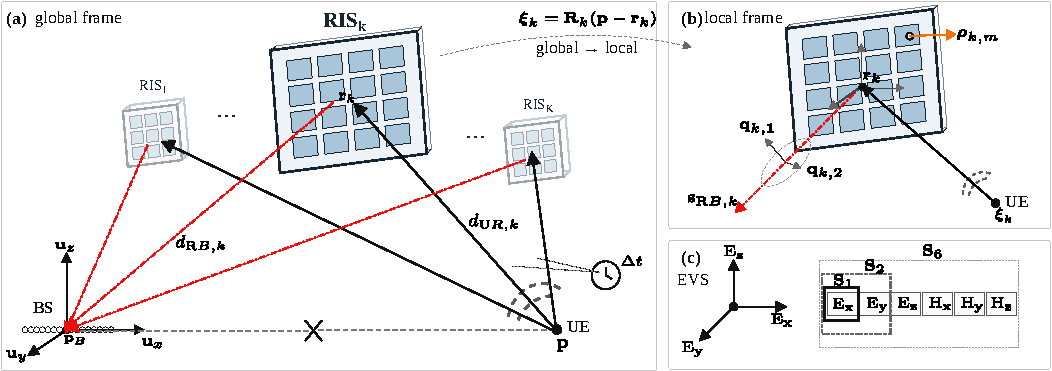
\includegraphics[width=\textwidth]{EVS_RIS_system_model-crop.pdf}
\caption{Cascaded geometry and parameterization: (a)~global frame,
    (b)~local frame of panel $k$, and (c)~six-component EVS element with the
    receiver modes.}
\label{fig:geometry}
\end{figure*}

\subsection{Calibrated RIS--BS Maxwell Factor}
\label{subsec:calibrated}

Calibration provides $\bp_B$, the BS phase center; $\br_k$ and
$\bR_k\in{\rm SO}(3)$, the center and the global-to-local rotation of panel
$k$; $\brho_{k,m}\in\R^3$, its element coordinates in that frame; and the BS
array geometry and EVS Maxwell response. The BS ULA lies along the global $x$ axis of the
orthonormal frame $\{\bu_x,\bu_y,\bu_z\}$ and
$\kappa=2\pi/\lambda_c$ is the center-frequency wavenumber.

The calibrated locations give the RIS--BS distance and propagation direction
of panel $k$,
\begin{equation}
	d_{{\rm RB},k}=\|\bp_B-\br_k\|_2,
	\qquad
	\bs_{{\rm RB},k}=\frac{\bp_B-\br_k}{d_{{\rm RB},k}},
	\label{eq:rbgeom}
\end{equation}
and, under the far-field RIS--BS model established above, a plane-wave panel
response and a BS steering vector,
\begin{align}
	\big[\ba_{{\rm RB},k}\big]_m
	&=e^{j\kappa\,\brho_{k,m}^{\mathsf T}\bR_k\bs_{{\rm RB},k}},\nonumber\\
	\big[\bv_{{\rm B},k}\big]_i
	&=e^{-j\kappa x_i\,\bu_x^{\mathsf T}\bs_{{\rm RB},k}},
	\label{eq:arb_vb}
\end{align}
with $x_i$ the $x$ coordinate of the $i$th BS element,
$\ba_{{\rm RB},k}\in\C^{M_R}$ and $\bv_{{\rm B},k}\in\C^{M_A}$.

The same direction fixes the polarization manifold: a transverse plane wave
along $\bs_{{\rm RB},k}$ has Maxwell pair
$(\bE,\bH)=(\bq,\bs_{{\rm RB},k}\times\bq)$ in impedance-normalized units, so
with any transverse basis
\begin{equation}
	\bq_{k,1}\in\bs_{{\rm RB},k}^{\perp},
	\quad \|\bq_{k,1}\|_2=1,
	\qquad
	\bq_{k,2}=\bs_{{\rm RB},k}\times\bq_{k,1},
	\label{eq:qbasis}
\end{equation}
the six-component
vector-sensor manifold~\cite{nehorai1994vector,khan2020sixcomponent}
specializes to the calibrated Maxwell--Jones block
\begin{equation}
	\bTheta_k^{(6)}=\begin{bmatrix}
	\bq_{k,1} & \bq_{k,2}\\[1pt]
	\bq_{k,2} & -\bq_{k,1}\end{bmatrix}\in\C^{6\times2},
	\label{eq:Theta}
\end{equation}
whose columns satisfy
$[\bTheta_k^{(6)}]^{\mathsf H}\bTheta_k^{(6)}=2\bI_2$; a rotation
$\bU\in{\rm SO}(2)$ of the transverse basis sends
$\bTheta_k^{(6)}\mapsto\bTheta_k^{(6)}\bU$ and is absorbed by
$\bx_k\mapsto\bU^{\mathsf T}\bx_k$. A fixed selection matrix
$\bS_{\rm mode}\in\R^{d_{\rm evs}\times6}$,
\begin{equation}
	\bS_1=\begin{bmatrix}1 & \mathbf 0\end{bmatrix},
	\quad
	\bS_2=\begin{bmatrix}\bI_2 & \mathbf 0\end{bmatrix},
	\quad
	\bS_6=\bI_6,
	\label{eq:smode}
\end{equation}
with $d_{\rm evs}\in\{1,2,6\}$ for the scalar, dual-polarized and full-EVS
receiver modes of Fig.~\ref{fig:geometry}(c), gives
$\bTheta_k^{({\rm mode})}\triangleq\bS_{\rm mode}\bTheta_k^{(6)}
\in\C^{d_{\rm evs}\times2}$ and the receive dimension $I=d_{\rm evs}M_A$.

The calibrated receive block
$\bBm_k\triangleq\bv_{{\rm B},k}\otimes\bTheta_k^{({\rm mode})}\in\C^{I\times2}$
is known before UE estimation and satisfies
$\partial\bBm_k/\partial\bchi=\mathbf0$; only the Jones-domain coefficients
$\bx_k\in\C^2$ of \eqref{eq:roadmap} remain unknown, each being the effective
polarization state launched toward the BS after reflection rather than the UE
antenna state.

\subsection{UE--RIS Near-Field and Common-Clock Factor}
\label{subsec:defchain}

The unknown nonlinear parameter collects the UE position and common clock
offset, $\bchi=[\bp^{\mathsf T},\Delta t]^{\mathsf T}
=[x,y,z,\Delta t]^{\mathsf T}\in\R^4$, with $\bp\in\mathcal P$ a known closed
service box and $\Delta t\in\mathcal T$, where $\mathcal T$ is a known closed
interval with $|\mathcal T|<1/\Delta f$, the unambiguous delay period. Every cascaded delay is
the geometric propagation time plus the same offset~\cite{fascista2022rissync,gong2024async,yan2025ris}.
In the $k$th panel frame (Fig.~\ref{fig:geometry}(b)),
$\bxi_k(\bp)=\bR_k(\bp-\br_k)$ and
\begin{equation}
	d_{{\rm UR},k}(\bp)=\|\bxi_k(\bp)\|_2=\|\bp-\br_k\|_2,
	\quad
	\bs_{{\rm UR},k}(\bp)=\frac{\bxi_k(\bp)}{d_{{\rm UR},k}(\bp)},
	\label{eq:urgeom}
\end{equation}
since $\bR_k$ is a rotation. Element $m$ of panel $k$
applies the scalar Jones response $e^{j\omega_{k,t,m}}\bI_2$ at configuration
$t$, so no polarization mixing occurs; with the prescribed constant-modulus
training $[\bOmega_k]_{t,m}=e^{j\omega_{k,t,m}}/\sqrt{M_R}$,
$\bOmega_k\in\C^{T\times M_R}$~\cite{lin2021tensor}, the near-field
dependence is captured by the RIS response
\begin{align}
	\bg_k(\bp) &= \ba_{{\rm RB},k}\odot\ba^{\rm NF}_{{\rm UR},k}(\bp)
	\in\C^{M_R},\nonumber\\
	\bh_k(\bp) &= \bOmega_k\,\bg_k(\bp)\in\C^{T},
	\label{eq:hk}
\end{align}
where
\begin{align}
	\big[\ba^{\rm NF}_{{\rm UR},k}(\bp)\big]_m
	&= e^{-j\kappa\delta_{k,m}(\bp)},
	\quad \ba^{\rm NF}_{{\rm UR},k}\in\C^{M_R},\nonumber\\
	\delta_{k,m}(\bp)
	&= \big\|\bxi_k(\bp)-\brho_{k,m}\big\|_2
	- d_{{\rm UR},k}(\bp).
	\label{eq:delta}
\end{align}
Equation~\eqref{eq:delta} retains the exact spherical-wave phase across the
panel aperture (Fig.~\ref{fig:geometry}(b)); the Fresnel approximation enters
only in Phase-I proposal generation (Section~\ref{subsec:beamspace}).

Combining \eqref{eq:rbgeom} and \eqref{eq:urgeom}, the cascaded delay and its
OFDM phase ramp on the tone grid
$f_n=f_c+\big(n-\tfrac{N-1}{2}\big)\Delta f$, $n=0,\ldots,N-1$, are
\begin{align}
	\tau_k(\bp,\Delta t)
	&= \underbrace{\frac{d_{{\rm UR},k}(\bp) + d_{{\rm RB},k}}{c_0}}_{
	\textstyle \tau_{g,k}(\bp)} + \Delta t,\nonumber\\
	\bd_k(\bp,\Delta t)
	&= \Big[\,e^{-j2\pi\left(n-\frac{N-1}{2}\right)\Delta f\,
	\tau_k(\bp,\Delta t)}\,\Big]_{n=0}^{N-1}\in\C^N,
	\label{eq:dk}
\end{align}
with the tone-independent phase $e^{-j2\pi f_c\tau_k}$ absorbed into the
path gain. In contrast to the
frequency-dependent spatial manifold of~\cite{yang2024nfris}, the present
model carries the wideband dependence entirely through \eqref{eq:dk}. For an
inter-element path difference $\Delta L$ in a spatial response, the phase
neglected in (A4) is $\epsilon_{\rm sq}=\pi B_{\rm occ}\max|\Delta L|/c_0$.

The bracketed factor of \eqref{eq:roadmap} is the per-panel sensing block,
which by associativity of the Kronecker product also takes the
form~\eqref{eq:premise},
\begin{align}
	\bA_k(\bchi)
	&= \bh_k(\bp)\otimes\bd_k(\bp,\Delta t)\otimes\bBm_k\nonumber\\
	&= \bc_k(\bchi)\otimes\bTheta_k^{({\rm mode})}\in\C^{M\times2},
	\label{eq:Ak}
\end{align}
where $\bc_k(\bchi)=\bh_k(\bp)\otimes\bd_k(\bp,\Delta t)\otimes
\bv_{{\rm B},k}\in\C^{TNM_A}$ is the space--frequency factor.

Arranging the $I$ receive channels against the $N$ subcarriers at
configuration $t$ gives
\begin{equation}
	\bY_t=\sum_{k=1}^{K}[\bh_k(\bp)]_t\,(\bBm_k\bx_k)\,
	\bd_k(\bp,\Delta t)^{\mathsf T}+\bN_t,
	\label{eq:obsmat}
\end{equation}
where $t=1,\ldots,T$, $\bY_t\in\C^{I\times N}$ and $\bN_t$ is the noise
block. The grouping $\bh_k\otimes\bd_k\otimes\bBm_k$ exposes the receive
subspace used in Section~\ref{sec:algorithm};
$\bc_k\otimes\bTheta_k^{({\rm mode})}$ isolates receiver-mode selection for
Section~\ref{sec:analysis}.

\subsection{Observation and Estimation Problem}
\label{subsec:obsmodel}

Stacking the panels as
$\bA(\bchi)=[\bA_1(\bchi),\ldots,\bA_K(\bchi)]\in\C^{M\times 2K}$ and
vectorizing the $\bY_t$ in the same order writes \eqref{eq:roadmap} as
\begin{equation}
	\by = \bmu(\bchi,\bx) + \bn = \bA(\bchi)\,\bx + \bn,
	\qquad
	\bn\sim\mathcal{CN}(\mathbf 0,\sigma^2\bI_M),
	\label{eq:obs}
\end{equation}
where the noise is white across receive channels, subcarriers and RIS
configurations, and its power $\sigma^2$ is unknown to the estimator. The
unknown Jones-domain coefficient of path $k$
is $\bx_k=\beta_k\be_k\in\C^2$, stacked as
$\bx=[\bx_1^{\mathsf T},\ldots,\bx_K^{\mathsf T}]^{\mathsf T}\in\C^{2K}$,
where the complex gain $\beta_k$ absorbs path loss, RIS efficiency and the
center-frequency phase of the cascade and $\be_k$ is a unit Jones state
(angular parameterization in Table~\ref{tab:params}). Both factors are flat over the
occupied band and only their product is identifiable, so the estimator
treats $\bx_k$ as a free $\C^2$ nuisance.

Profiling $\sigma^2$ out of the white-Gaussian log-likelihood gives
$\widehat\sigma^2=\|\by-\bA(\bchi)\bx\|_2^2/M$, and the concentrated
log-likelihood is strictly decreasing in the residual energy, so maximum-likelihood (ML)
estimation of $(\bchi,\bx)$ is the least-squares problem
\begin{equation}
	\min_{\bp\in\mathcal P,\ \Delta t\in\mathcal T,\ \bx\in\C^{2K}}
	\big\|\by-\bA(\bp,\Delta t)\,\bx\big\|_2^2.
	\label{eq:ml_problem}
\end{equation}
The $2K$ Jones coefficients enter linearly and admit closed-form
elimination; position and clock enter nonlinearly through
\eqref{eq:delta} and \eqref{eq:dk}, leaving \eqref{eq:ml_problem} nonconvex
in four real coordinates.

\section{Proposed Estimator: Sufficient Acquisition and Certified Clock Profiling}
\label{sec:algorithm}

Direct optimization of \eqref{eq:ml_problem} must address panel association,
near-field basin acquisition, the $2K$ linear Jones coefficients and the common
clock simultaneously. We separate them with a two-phase estimator. Phase~I,
\emph{Maxwell--Kronecker sufficient compression with common-geometry
initialization} (MKSC-GI), projects onto the calibrated Maxwell receive
subspace, recovers and associates the cascaded factors, and fuses the
panel-local estimates into one common position initializer. Phase~II,
\emph{common-clock orbit-profiled Jones variable projection} (CCOP-JVP),
eliminates the Jones coefficients analytically and refines position and
clock by certified profiling along the exact clock orbit.
Algorithm~\ref{alg:mksc_ccop} collects both phases, with each step citing its
corresponding derivation. In the algorithm, ESPRIT denotes estimation of
signal parameters via rotational invariance techniques; DFT and FFT denote
the discrete and fast Fourier transforms, respectively.

\begin{algorithm}[!t]
\footnotesize
\caption{MKSC-GI-Initialized CCOP-JVP}
\label{alg:mksc_ccop}
\begin{algorithmic}[1]
\REQUIRE $\{\bY_t\}_{t=1}^{T}$, calibrated infrastructure, $K$,
$\mathcal P$, $\mathcal T$
\STATE \textbf{Phase~I: MKSC-GI}
\STATE Compress receive index: $\bY_{{\rm d},t}=\bQ_S^{\mathsf H}\bY_t$,
$I\!\to\!r\le2K$ \hfill\eqref{eq:calibsub}
\STATE Delay poles $\{\hat z_k\}$ by ESPRIT on the tone axis
\hfill\eqref{eq:shift}
\STATE Coupled factors $\hat\bF$ by one loaded weighted
least-squares (WLS) solve
\hfill\eqref{eq:coupledls_short}
\STATE Rank-one split $\to(\tilde\ba_j,\tilde\bt_j,\varrho_j)$
\hfill\eqref{eq:split_rank1}
\STATE Dechirped 2-D DFT proposals for all panel--column pairs
\hfill\eqref{eq:fresnel},\,\eqref{eq:Jris_short}
\STATE Two-tier permutation search with exact shortlist rescoring
\hfill\eqref{eq:assoc_perm}
\STATE Fuse by $J_{\rm geom}$; select by clock spread
\hfill\eqref{eq:Jgeom_short}
\STATE Jones-state anchors $\{\hat\be_k\}$ refreshed at $\hat\bp_{\rm GI}$
\hfill\eqref{eq:refresh_short}
\STATE Select Phase-II position initializer $\hat\bp_{\rm I}$ by clock--geometry consistency
\STATE \textbf{Phase~II: CCOP-JVP}
\REPEAT
\STATE Clock-profile coefficients $\{\gamma_\ell(\bp)\}$; FFT-seeded
candidates \hfill\eqref{eq:clock_coeff}
\STATE Branch and bound over $\Delta t$ until
$g_{\rm cert}\!\le\!\epsilon_{\rm clk}$ or cap \hfill\eqref{eq:bound_short}
\STATE Update $\bp$ by envelope gradient (safeguard if ambiguous)
\hfill\eqref{eq:envelope}
\UNTIL{outer convergence}
\STATE Profiled Jones coefficients $\hat\bx=\bG_\lambda^{\dagger}\bb$
\hfill\eqref{eq:vp_short}
\RETURN $(\hat\bp,\widehat{\Delta t},\hat\bx)$ and $g_{\rm cert}$
\end{algorithmic}
\end{algorithm}

\subsection{Maxwell--Kronecker Factor Recovery}

\textit{1) Sufficient compression and delay-pole recovery:}
The calibrated receive blocks in \eqref{eq:Ak} span
\begin{equation}
 \mathcal S_R=\sum_{k=1}^{K}\coll(\bBm_k)=\coll(\bPsi),
 \quad \bPsi=[\bBm_1,\ldots,\bBm_K],
 \label{eq:calibsub}
\end{equation}
with $r=\rank\bPsi\le2K$. An orthonormal basis $\bQ_S\in\C^{I\times r}$
depends only on calibration and satisfies
$\bQ_S\bQ_S^{\mathsf H}\bBm_k=\bBm_k$ for every panel. Projection onto this
basis gives
\begin{equation}
 \bY_{{\rm d},t}=\bQ_S^{\mathsf H}\bY_t
 =\sum_{k=1}^{K}[\bh_k(\bp)]_t\,\ba_k\,
 \bd_k(\bp,\Delta t)^{\mathsf T}+\bQ_S^{\mathsf H}\bN_t,
 \label{eq:obsmat_c}
\end{equation}
where $\ba_k=\bQ_S^{\mathsf H}\bBm_k\bx_k$.
Theorem~\ref{thm:compress} establishes sufficiency. In the reference scene,
the projection reduces the receive dimension from $I=96$ to $r=6$, discarding
noise-only directions while retaining white noise in the compressed
coordinates.

Each delay contributes the pole $z_k=e^{-j2\pi\Delta f\tau_k}$.
The centered tone grid adds only a nonzero column scalar:
$[\bd_k]_n=e^{j\pi(N-1)\Delta f\tau_k}z_k^n$.
Rearranging the compressed channel--configuration pairs as snapshots gives
\begin{equation}
 \bY_f=\sum_{k=1}^{K}\bd_k\,\bw_k^{\mathsf T}+\bN_f\in\C^{N\times rT},
 \qquad \bw_k=\ba_k\otimes\bh_k(\bp).
 \label{eq:freqsnap}
\end{equation}
For $\bD=[\bd_1,\ldots,\bd_K]$, removing its last or first row gives
$\underline{\bD}$ or $\overline{\bD}$, respectively, with
\begin{equation}
 \overline{\bD}=\underline{\bD}\,\boldsymbol\Phi,
 \qquad \boldsymbol\Phi=\diag(z_1,\ldots,z_K).
 \label{eq:shift}
\end{equation}
Distinct delays modulo $1/\Delta f$, $N\ge K+1$ and the snapshot-rank
condition of Theorem~\ref{thm:compress}(iv) permit recovery by
forward--backward total-least-squares ESPRIT
\cite{gong2026aimdf}, with estimated poles projected onto the
unit circle.

\textit{2) Coupled factor recovery:}
With the estimated delays fixed, we recover
$\bF=[\bw_1,\ldots,\bw_K]\in\C^{rT\times K}$ from the rearranged data
$\bY_{rT,N}$ by
\begin{equation}
 \hat\bF=\arg\min_{\bF}
 \big\|(\bY_{rT,N}-\bF\bD^{\mathsf T})\bW^{1/2}\big\|_F^2
 +\lambda_\tau\|\bF\|_F^2,
 \label{eq:coupledls_obj}
\end{equation}
or, equivalently, one $K\times K$ solve:
\begin{equation}
 \hat\bF=\bY_{rT,N}\bW\bD^{\ast}
 (\bD^{\mathsf T}\bW\bD^{\ast}+\lambda_\tau\bI)^{-1}.
 \label{eq:coupledls_short}
\end{equation}
The diagonal entries of $\bW=\diag(w_n)$ are the anti-diagonal
multiplicities $w_n=\#\{(p,\ell):p+\ell=n\}$ of the $P\times L$ Hankel
lift of the tone axis ($P+L-1=N$), and
$\lambda_\tau=10^{-6}\tr(\bD^{\mathsf T}\bW\bD^{\ast})/K+10^{-12}$;
solving in the lifted domain gives the same linear system. The window weights
this factor recovery only: the poles of \eqref{eq:shift} are estimated from the full
$N$-tone aperture, unsmoothed.
After column $j$ is reshaped as an $r\times T$ matrix with the receive index
running slowest, its leading singular triplet gives
\begin{equation}
 \tilde\ba_j=\sqrt{\sigma_{1,j}}\,\bQ_S\bu_{1,j},\quad
 \tilde\bt_j=\sqrt{\sigma_{1,j}}\,\bv_{1,j}^{\ast},\quad
 \varrho_j=\frac{\sigma_{2,j}}{\sigma_{1,j}}.
 \label{eq:split_rank1}
\end{equation}
For exact poles and zero loading, the noiseless factors of the generating
panel $k$ satisfy
\begin{equation}
 \tilde\ba_j=c_j\,\bBm_k\bx_k,\qquad
 \tilde\bt_j=c_j'\,\bh_k(\bp),
 \label{eq:factor_meaning}
\end{equation}
where $c_j,c_j'\ne0$ encode a scale and phase ambiguity, so subsequent
criteria must be scale invariant; $\varrho_j$ measures departure from rank
one and weights the common-geometry fit.

\textit{3) Physical panel association:}
For column $j$ and candidate panel $k$, the score combines calibrated
receive-subspace and spherical-wave consistency:
\begin{equation}
 s_{j,k}=
 \frac{\|\bPi^{\perp}_{\bBm_k}\tilde\ba_j\|}{\|\tilde\ba_j\|}
 +\min_{\boldsymbol\eta\in\mathcal E_k}
 \frac{\|\bPi^{\perp}_{\bh_k(\boldsymbol\eta)}\tilde\bt_j\|}
 {\|\tilde\bt_j\|}.
 \label{eq:assoc_score}
\end{equation}
The vector $\boldsymbol\eta=(d,u,v)$ contains a candidate range and the first two
direction cosines in panel $k$'s local frame; $\mathcal E_k$ is its search
box, and $\bh_k$ is the exact response \eqref{eq:hk}.
The minimization over $\mathcal E_k$ is initialized by the beam-space
proposals of Section~\ref{subsec:beamspace} and is evaluated for all $K^2$
panel--column pairs before an association is fixed.
The minimizing range $\hat d_{j,k}$ implies a clock replica
$\widehat{\Delta t}_{j,k}=\hat\tau_j-(\hat d_{j,k}+d_{{\rm RB},k})/c_0$.
Each permutation is scored by
\begin{equation}
 C(\pi)=\sum_{j=1}^{K}s_{j,\pi(j)}
 +\frac{w_{\rm clk}}{t_0}
 [\,\mathrm{sd}(\pi)+e_{\mathcal T}(\pi)\,],
 \label{eq:assoc_perm}
\end{equation}
where $e_{\mathcal T}$ is the mean excursion outside $\mathcal T$,
$w_{\rm clk}=1/2$, $t_0=1$~ns, and
\begin{align}
 \mathrm{sd}(\pi)&=\Big[\tfrac1K\sum_{j=1}^{K}
 (\widehat{\Delta t}_{j,\pi(j)}-\overline{\Delta t}(\pi))^2
 \Big]^{1/2},\nonumber\\
 \overline{\Delta t}(\pi)&=\tfrac1K\sum_{j=1}^{K}
 \widehat{\Delta t}_{j,\pi(j)}.
 \label{eq:assoc_sd}
\end{align}
The common clock mean $\overline{\Delta t}(\pi)$ couples the assignments, so
this is not a linear assignment problem. A deterministic two-tier search ranks all $K!$
permutations using a cached coarse codebook, then re-scores only the best
two, $\pi_{(1)},\pi_{(2)}$, using exact spherical projection:
\begin{equation}
 \hat\pi=\arg\min_{\pi\in\{\pi_{(1)},\pi_{(2)}\}}C(\pi).
 \label{eq:assoc_two_tier}
\end{equation}
It returns the delay--factor triples
$\{\hat\tau_j,\tilde\ba_j,\tilde\bt_j;\hat\pi(j)\}$ indexed by their associated
panels for geometric acquisition.

\subsection{Beam-Space Acquisition and Common-Geometry Initialization}
\label{subsec:beamspace}

\textit{1) Panel-local beam-space acquisition:}
By \eqref{eq:factor_meaning} the factor $\tilde\bt_k$ that $\hat\pi$ assigns
to panel $k$ is $\bh_k$ up to an unknown scale. Its geometry is recovered
separately for each panel before the $K$ estimates are reconciled
into a common position by the scale-invariant fit
\begin{equation}
 J_{\rm RIS}(\boldsymbol\eta)
 =\|\bPi_{\bh_k(\boldsymbol\eta)}^\perp\tilde\bt_k\|^2
 =\|\tilde\bt_k\|^2-
 \frac{|\bh_k^{\mathsf H}(\boldsymbol\eta)\tilde\bt_k|^2}
 {\|\bh_k(\boldsymbol\eta)\|^2},
 \label{eq:Jris_short}
\end{equation}
with $\bh_k(\boldsymbol\eta)=\bOmega_k[\ba_{{\rm RB},k}\odot
\ba^{\rm NF}(\boldsymbol\eta)]$ over the panel-local coordinates
$\boldsymbol\eta$ defined above. A fixed-count angular dictionary of the polar
or beam-training kind~\cite{cui2022channel,zheng2025wideband} has a step size set
by the search box, not by the panel resolution $\lambda_c/D_{\rm ap}$, so the
dominant
angular search is moved to the element domain. The training code enters
$\bh_k$ only on the left, so moving $\bOmega_k^{\mathsf H}$ across and
splitting the Hadamard product gives
\begin{align}
 \bh_k^{\mathsf H}(\boldsymbol\eta)\tilde\bt_k
 &=\big[\ba_{{\rm RB},k}\odot\ba^{\rm NF}(\boldsymbol\eta)\big]^{\mathsf H}
 \big(\bOmega_k^{\mathsf H}\tilde\bt_k\big)
 =\big[\ba^{\rm NF}(\boldsymbol\eta)\big]^{\mathsf H}\tilde\bg_k,\nonumber\\
 \tilde\bg_k&=\ba_{{\rm RB},k}^{\ast}\odot
 (\bOmega_k^{\mathsf H}\tilde\bt_k).
 \label{eq:adjoint_short}
\end{align}
One adjoint pass fixes $\tilde\bg_k$ per panel and leaves
$\ba^{\rm NF}(\boldsymbol\eta)$ as the only $\boldsymbol\eta$-dependent factor
in the numerator of \eqref{eq:Jris_short}; the denominator admits no such
reduction and is evaluated exactly. Expanding \eqref{eq:delta} to second
order about the panel center, with
$\bu=[u,v,\sqrt{1-u^2-v^2}]^{\mathsf T}$ the unit direction from that center
to the UE in the panel frame,
\begin{equation}
	\delta_{k,m}\simeq-\brho_{k,m}^{\mathsf T}\bu
	+\frac{\|\brho_{k,m}\|^2-(\brho_{k,m}^{\mathsf T}\bu)^2}{2\tilde d},
	\label{eq:fresnel}
\end{equation}
so the paraxial dechirp $\tilde\bg_{k,\tilde d}[m]=\tilde\bg_k[m]
e^{j\kappa\|\brho_{k,m}\|^2/(2\tilde d)}$ removes the isotropic quadratic term
at trial range $\tilde d$ and leaves the plane-wave phase
$e^{j\kappa\brho_{k,m}^{\mathsf T}\bu}$, up to the direction-dependent
curvature $(\brho_{k,m}^{\mathsf T}\bu)^2/(2\tilde d)$. One zero-padded 2-D
DFT then scores all direction-cosine pairs at once on
a grid tracking the Rayleigh limit, requiring one transform per trial range
rather than an atom-by-atom dictionary scan. Because of the residual curvature,
\eqref{eq:fresnel} is used only to generate proposals: every retained angular
peak receives an exact spherical range scan and is re-scored by the full
\eqref{eq:Jris_short}, so the candidate set changes acquisition coverage and
cost but not the forward model. The candidate set for each experiment is stated in
Section~\ref{sec:simulation}.

\textit{2) Common-geometry fusion:}
Each panel-local estimate $\hat{\boldsymbol\eta}_k$ maps through the calibrated
panel pose back to a global position
$\hat\bp_k^{\rm loc}=\br_k+\bR_k^{\mathsf T}\bxi_k(\hat{\boldsymbol\eta}_k)$,
inverting $\bxi_k(\bp)=\bR_k(\bp-\br_k)$. These $K$ positions generally
disagree; the common-geometry stage replaces them by the single position that
best explains all $K$ training factors at once, each up to its own unknown
complex scale,
\begin{align}
 J_{\rm geom}(\bp)
 &=\min_{\balpha\in\C^K}\sum_{k=1}^K \varpi_k
 \|\tilde\bt_k-\alpha_k\bh_k(\bp)\|^2
 \label{eq:Jgeom_short}\\
 &=\sum_{k=1}^K \varpi_k\left[\|\tilde\bt_k\|^2-
 \frac{|\bh_k^{\mathsf H}(\bp)\tilde\bt_k|^2}{\|\bh_k(\bp)\|^2}\right],
 \nonumber
\end{align}
the second line following from the profiled scale
$\hat\alpha_k(\bp)=\bh_k^{\mathsf H}(\bp)\tilde\bt_k/\|\bh_k(\bp)\|^2$, so
only the component of $\tilde\bt_k$ orthogonal to $\coll(\bh_k)$ remains and
the gains need not be known. The weights
$\varpi_k=\max\{e^{-\varrho_k/\varrho_0},\varpi_{\min}\}$, with
$\varrho_0=1/2$ and $\varpi_{\min}=0.05$, down-weight a column
whose rank-one split is poor while keeping every panel in the fit. We minimize
\eqref{eq:Jgeom_short} with bounded L-BFGS-B~\cite{byrd1995lbfgsb} from
deterministic starts around
$\hat\bp_0=\clip_{\mathcal P}\{\median_k\hat\bp_k^{\rm loc}\}$. Among the
near-optimal minima, we select $\hat\bp_{\rm GI}$ as the one whose clock
replicas $\hat\tau_k-(\|\bp-\br_k\|+d_{{\rm RB},k})/c_0$ vary least.

\textit{3) Jones-state anchor refresh:}
At the selected $\hat\bp_{\rm GI}$, the $\lambda_k=0$ instance of the
certified clock profiler of Section~\ref{subsec:ccop} refreshes the Jones-state
anchors at a fixed position,
\begin{equation}
 (\widehat{\Delta t}_{\rm ref},\hat\bx_{\rm ref})=
 \arg\min_{\Delta t\in\mathcal T,\bx}
 \|\by-\bA(\hat\bp_{\rm GI},\Delta t)\bx\|^2.
 \label{eq:refresh_short}
\end{equation}
With $\hat\bx_{{\rm ref},k}$ the $k$th two-entry block of $\hat\bx_{\rm ref}$,
the anchor is $\hat\be_k=\hat\bx_{{\rm ref},k}/\|\hat\bx_{{\rm ref},k}\|_2$,
obtained at the common position from a conditional clock solve with an
optimality-gap certificate of the same form. The implementation chooses the
Phase-II position initializer $\hat\bp_{\rm I}$ from $\hat\bp_{\rm GI}$, the mean and
coordinatewise median of the panel-local positions, and their $K$
leave-one-out means by minimizing the median absolute deviation of the implied
panel clocks plus the median position discrepancy divided by $c_0$. The
refreshed anchors initialize the Phase-II directional regularizer.

\subsection{Common-Clock Orbit-Profiled Jones Variable Projection}
\label{subsec:ccop}

\textit{1) Unitary clock orbit and directional Jones regularization:}
Phase~II refines the Phase-I initializer using the exact forward model
underlying \eqref{eq:ml_problem} and a directional Jones penalty.
Its $2K$ Jones coefficients enter linearly and are eliminated in
closed form by variable projection, leaving four
nonlinear coordinates. By Theorem~\ref{thm:compress}, the implementation
evaluates the criterion on the compressed observation of Phase~I without
approximation. The common clock is the only nonlinear
coordinate along which the likelihood admits an exact unitary symmetry. Let
$\bA_0(\bp)\triangleq\bA(\bp,0)$ and
$\bD_{\rm clk}(\Delta t)=\diag([e^{-j2\pi(n-\frac{N-1}{2})\Delta f\Delta t}]_{n=0}^{N-1})$.
Then
\begin{align}
 \bU_{\rm clk}(\Delta t)&=\bI_T\otimes\bD_{\rm clk}(\Delta t)\otimes\bI_I,
 \nonumber\\
 \bA(\bp,\Delta t)&=\bU_{\rm clk}(\Delta t)\bA_0(\bp),
 \label{eq:orbit_short}\\
 \bA^{\mathsf H}\bA
 &=\bA_0^{\mathsf H}\bU_{\rm clk}^{\mathsf H}\bU_{\rm clk}\bA_0\nonumber\\
 &=\bA_0^{\mathsf H}\bA_0\triangleq\bG_0(\bp).
 \label{eq:clock_gram}
\end{align}
Phase~II uses the clock-independent, Gram-scaled penalty
\begin{equation}
 \bR_{\rm dir}(\bp)=\blkdiag_k\left[
 \lambda_k\tfrac12\tr\bG_{0,kk}(\bp)\,\bPi_{\hat\be_k}^{\perp}\right],
 \label{eq:Rdir_short}
\end{equation}
with $\lambda_k=1$ throughout (Remark~\ref{rem:peb_reading}) and
$\bR_{{\rm dir},kk}\hat\be_k=\mathbf0$, leaving the anchor direction and
complex gain free. The diagonal data blocks satisfy
\begin{equation}
	\bG_{0,kk}=N M_A\|\bh_k(\bp)\|^2\,
	[\bTheta_k^{({\rm mode})}]^{\mathsf H}\bTheta_k^{({\rm mode})}.
	\label{eq:g0block}
\end{equation}
The receiver mode determines how many Jones coordinates are observable,
\begin{equation}
	\rank\bG_{0,kk}=\rank\bTheta_k^{({\rm mode})}
	=\min\{d_{\rm evs},2\},
	\label{eq:g0rank}
\end{equation}
for generic panel orientations. The scalar receiver mode leaves one Jones
coordinate per panel unobserved. For the full normal matrix
$\bG_\lambda=\bG_0+\bR_{\rm dir}$, positive definiteness is characterized by
\begin{equation}
	\bG_\lambda\succ\mathbf0
	\iff
 \ker(\bG_0)\cap\ker(\bR_{\rm dir})=\{\mathbf0\}.
	\label{eq:glambda_pd}
\end{equation}
\textit{2) Jones variable projection and the trigonometric clock profile:}
Phase~II accordingly minimizes the penalized exact-model criterion
\begin{equation}
 J(\bp,\Delta t,\bx)=\|\by-\bA(\bp,\Delta t)\bx\|_2^2
 +\bx^{\mathsf H}\bR_{\rm dir}(\bp)\bx.
 \label{eq:penalized_short}
\end{equation}
Theorem~\ref{thm:clock} establishes exact nesting of this criterion, which
reduces to \eqref{eq:ml_problem} at $\lambda_k=0$.
Substituting \eqref{eq:orbit_short} into \eqref{eq:penalized_short} and using
$\bU_{\rm clk}^{\mathsf H}\bU_{\rm clk}=\bI$ makes $J$ a quadratic in $\bx$
whose Hessian is independent of the clock,
\begin{equation}
 J=\|\by\|_2^2-2\Real\{\bx^{\mathsf H}\bb(\bp,\Delta t)\}
 +\bx^{\mathsf H}\bG_\lambda(\bp)\bx,
 \label{eq:jquad}
\end{equation}
with $\bb=\bA_0^{\mathsf H}\bU_{\rm clk}^{\mathsf H}\by$. The
Wirtinger stationarity condition
$\partial J/\partial\bx^{\ast}=\bG_\lambda\bx-\bb=\mathbf0$ removes all
$2K$ Jones coefficients in one step; for $\bG_\lambda\succ\mathbf0$,
\begin{align}
 \hat\bx&=\bG_\lambda^{-1}\bb,
 \quad Q(\bp,\Delta t)=\bb^{\mathsf H}\bG_\lambda^{-1}\bb,\nonumber\\
 F(\bp,\Delta t)&\triangleq\min_{\bx\in\C^{2K}}J=\|\by\|_2^2-Q.
 \label{eq:vp_short}
\end{align}
At singular positions, the implementation uses $\bG_\lambda^{\dagger}\bb$ as the
minimum-norm Jones solution, without adding a ridge. Since
$\bb\in\coll(\bG_\lambda)$, this preserves the fixed-position criterion
and the polynomial clock profile below. The 3-D outer objective is
\begin{equation}
 \widetilde F(\bp)=\|\by\|^2-
 \max_{\Delta t\in\mathcal T}Q(\bp,\Delta t).
 \label{eq:nested_short}
\end{equation}
We group the sufficient-statistic correlations by tone as
$\bb(\bp,\Delta t)=\sum_{n=0}^{N-1}\bu_n(\bp)
e^{j2\pi(n-\frac{N-1}{2})\Delta f\Delta t}$. Because
$\bG_\lambda^{-1}$ is clock-independent, substitution into $Q$ gives
\begin{align}
 Q(\bp,\Delta t)
 &=\sum_{n=0}^{N-1}\sum_{n'=0}^{N-1}
 \bu_n^{\mathsf H}\bG_\lambda^{-1}\bu_{n'}\,
 e^{j2\pi(n'-n)\Delta f\Delta t}\nonumber\\
 &=\sum_{\ell=-(N-1)}^{N-1}\gamma_\ell(\bp)
 e^{j2\pi\ell\Delta f\Delta t},\quad \gamma_{-\ell}=\gamma_\ell^\ast,
 \label{eq:trig_short}\\
 \gamma_\ell(\bp)
 &=\sum_{n=0}^{N-1-\ell}\bu_n^{\mathsf H}(\bp)
 \bG_\lambda^{-1}(\bp)\bu_{n+\ell}(\bp),
 \label{eq:clock_coeff}
\end{align}
for $\ell=0,\ldots,N-1$. This representation makes $Q$ a real trigonometric
polynomial of degree at most $N-1$. The factorization of $\bG_\lambda$ at each position is
reused for coefficient assembly and FFT-seeded clock candidates; subsequent
interval tests evaluate only the polynomial and its derivatives. At fixed
$\bp$, write $q_{\bp}(s)=Q(\bp,s)$ for clock offset $s$. Differentiating
twice gives
\begin{equation}
 |q_{\bp}''(s)|\le(2\pi\Delta f)^2
 \sum_{\ell=-(N-1)}^{N-1}\ell^2|\gamma_\ell|\triangleq L_2.
 \label{eq:clock_curvature}
\end{equation}
For an interval centered at $s_c$ with half-width $r_s$, Taylor expansion
yields
\begin{equation}
 q_{\bp}(s)\le q_{\bp}(s_c)+|q_{\bp}'(s_c)|r_s+\tfrac12L_2r_s^2.
 \label{eq:bound_short}
\end{equation}
\textit{3) Certified clock maximization and outer refinement:}
Branch-and-bound maintains \eqref{eq:bound_short} over $\mathcal T$ and
returns an incumbent with
$q_{\bp}(\Delta t^\star(\bp))-q_{\bp}(\widehat{\Delta t}(\bp))
\le U-q_{\bp}(\widehat{\Delta t}(\bp))
\triangleq g_{\rm cert}$, where $U=\max\{U_{\rm act},U_{\rm pru}\}$ is the
largest bound over surviving and incumbent-pruned intervals. Subdivision stops
once $g_{\rm cert}\le\epsilon_{\rm clk}$ or $2\times10^4$ subdivisions are
reached, where $\epsilon_{\rm clk}=M\epsilon_{\rm abs}+\epsilon_{\rm rel}
\max\{\|\by\|^2,|Q_{\rm inc}|\}$, $Q_{\rm inc}$ is the incumbent score
when subdivision begins, $\epsilon_{\rm abs}=10^{-12}$ and
$\epsilon_{\rm rel}=10^{-10}$. At
every outer position, the returned clock solution
has a deterministic gap certificate and is $\epsilon_{\rm clk}$-optimal
whenever termination is by tolerance, as Theorem~\ref{thm:clock}(iii) states. For a
unique interior maximizer $\Delta t^\star(\bp)$ of $Q(\bp,\cdot)$, the exact
outer profile satisfies
\begin{equation}
 \nabla_{\bp}\widetilde F(\bp)
 =-\nabla_{\bp}Q(\bp,\Delta t)\big|_{\Delta t=\Delta t^\star(\bp)}.
	\label{eq:envelope}
\end{equation}
The outer position search starts from $\hat\bp_{\rm I}$ and approximates the envelope
gradient by evaluating the right-hand side of \eqref{eq:envelope} at the
computed $\widehat{\Delta t}(\bp)$. A derivative-free
safeguard is used when the clock solve does not meet its tolerance or
the maximizing branch is ambiguous. Phase~II outputs
$(\hat\bp,\widehat{\Delta t},\hat\bx)$ together with a gap certificate for
each conditional clock solve evaluated.


\section{Structural Analysis and Guarantees}
\label{sec:analysis}

We first state the reference free-Jones EFIM and its local rank condition,
then establish C1--C3 under their stated conditions.

\subsection{Reference Information and Identifiability}
Let $\bD_\chi=[\partial(\bA\bx)/\partial\chi_i]_{i=1}^4$. Eliminating the
unknown complex Jones coefficients from the white-Gaussian Fisher
information matrix gives the free-Jones equivalent Fisher information
matrix (EFIM), the reference information of the unpenalized data model,
\begin{equation}
 \bJ_\chi^{\rm free}=\frac{2}{\sigma^2}
 \Real\{\bD_\chi^{\mathsf H}\bPi_{\bA}^{\perp}\bD_\chi\}.
 \label{eq:efim_short}
\end{equation}
The projector has a direct interpretation: a geometric perturbation
$\bD_\chi\,\delta\bchi$ with $\delta\bchi\in\R^4$ is indistinguishable from a
Jones perturbation exactly when it lies in $\coll(\bA)$, that is when
$\bPi_{\bA}^{\perp}\bD_\chi\,\delta\bchi=\mathbf0$.
The first-order condition for local position--clock identifiability is
obtained by stacking the real and imaginary parts of that map:
\begin{equation}
 \widetilde\bD_\chi=\begin{bmatrix}
 \Real\{\bPi_{\bA}^{\perp}\bD_\chi\}\\
 \Imag\{\bPi_{\bA}^{\perp}\bD_\chi\}\end{bmatrix},
 \qquad \rank_{\R}\widetilde\bD_\chi=4.
 \label{eq:rankcond}
\end{equation}
Since
$\widetilde\bD_\chi^{\mathsf T}\widetilde\bD_\chi
=\Real\{\bD_\chi^{\mathsf H}\bPi_{\bA}^{\perp}\bD_\chi\}$, this condition is
equivalent to $\bJ_\chi^{\rm free}\succ\mathbf0$. The EFIM then yields the
position error bound (PEB) and clock error bound (CEB), defined as
${\rm PEB}=\sqrt{\tr[(\bJ_p^{\rm eff})^{-1}]}$ and
${\rm CEB}=\sqrt{[(\bJ_\chi^{\rm free})^{-1}]_{4,4}}$, with
$\bJ_p^{\rm eff}=\bJ_{pp}-\bJ_{pt}J_{tt}^{-1}\bJ_{tp}$. The blocks
$\bJ_{pp}\in\R^{3\times3}$, $\bJ_{pt}=\bJ_{tp}^{\mathsf T}\in\R^{3\times1}$,
and $J_{tt}\in\R$ are the position, cross and clock blocks of
$\bJ_\chi^{\rm free}$. The Jacobian of the
cascaded delays in \eqref{eq:dk} is
\begin{equation}
	\bD_\tau(\bp)
	=\frac{\partial[\tau_1,\ldots,\tau_K]^{\mathsf T}}
	{\partial\bchi^{\mathsf T}}
	=\begin{bmatrix}
	c_0^{-1}\bs_{{\rm UR},1}^{\mathsf T}\bR_1 & 1\\
	\vdots & \vdots\\
	c_0^{-1}\bs_{{\rm UR},K}^{\mathsf T}\bR_K & 1
	\end{bmatrix}\in\R^{K\times4}.
	\label{eq:delayjac}
\end{equation}
Row differencing removes the all-ones clock column. At $K=3$,
$\rank\bD_\tau\le3<4$, so the cascaded delays cannot identify $\bchi$ by
themselves. Additional position sensitivity comes from the aperture phase of
\eqref{eq:delta}: with
$\bs_{k,m}=(\bxi_k-\brho_{k,m})/\|\bxi_k-\brho_{k,m}\|_2$, the unit vector
from element $m$ to the UE,
\begin{equation}
	\frac{\partial\delta_{k,m}}{\partial\bp}
	=\bR_k^{\mathsf T}\big[\bs_{k,m}(\bp)-\bs_{{\rm UR},k}(\bp)\big],
	\label{eq:apertjac}
\end{equation}
the deviation of each element's bearing from the panel bearing that
\eqref{eq:delayjac} already carries. This tangent scales as
$O(\|\brho_{k,m}\|/d_{{\rm UR},k})$ and weakens toward the far-field limit.
Whether it restores rank four is not settled by counting; it requires
conditions on the RIS codes, wavefront curvature across the panel aperture
and geometry. After
complex-scale elimination the projected tangents
$\bPi_{\bh_k}^{\perp}[\partial\bh_k/\partial x,\partial\bh_k/\partial y,
\partial\bh_k/\partial z]$ retain the phase slope and curvature of
\eqref{eq:delta}. This rank test is local and conditional on the panel
association. Pseudoinverse projectors cover the rank-deficient Jones blocks of
\eqref{eq:g0rank}.

\subsection{C1: Maxwell--Jones Information Splitting}
Both parts of C1 rest on one identity: because $\bA_k$ is a Kronecker
product, so is its projector, and the complement separates into a
polarization-orthogonal component along the geometric factor and a
geometry-orthogonal component acting identically on every polarization.

\begin{lemma}[Kronecker projector splitting]
\label{lem:kron}
Let $\bc\neq\mathbf0$ and $\bTheta\neq\mathbf0$ be arbitrary, with
$\bP_{\bTheta}=\bTheta\bTheta^{\dagger}$. With $\bA=\bc\otimes\bTheta$,
\begin{equation}
 \bPi_{\bA}^{\perp}
 =\bP_{\bc}\otimes\bPi_{\bTheta}^{\perp}+\bPi_{\bc}^{\perp}\otimes\bI,
 \qquad \bP_{\bc}=\frac{\bc\bc^{\mathsf H}}{\|\bc\|^2}.
 \label{eq:kronsplit}
\end{equation}
\end{lemma}

\begin{IEEEproof}
$\bA^{\mathsf H}\bA=(\bc^{\mathsf H}\bc)(\bTheta^{\mathsf H}\bTheta)$ and
$\bA^{\dagger}=\bc^{\dagger}\otimes\bTheta^{\dagger}$, so
$\bP_{\bA}=\bP_{\bc}\otimes\bP_{\bTheta}$. Expanding
$\bI=(\bP_{\bc}+\bPi_{\bc}^{\perp})\otimes(\bP_{\bTheta}
+\bPi_{\bTheta}^{\perp})$ and subtracting $\bP_{\bA}$ gives
\eqref{eq:kronsplit}. No rank assumption is used, so the identity also holds
when a receiver mode makes the retained Jones block rank deficient.
\end{IEEEproof}

\begin{theorem}[C1: Maxwell--Jones information splitting]
\label{thm:split}
\textbf{(i) Information consequence.} For one panel, write
$\bA=\bc\otimes\bTheta$, $\boldsymbol{\zeta}=\bTheta\bx$,
$\dot\bc_i=\partial\bc/\partial\chi_i$, and
$\dot{\boldsymbol{\zeta}}_i=(\partial\bTheta/\partial\chi_i)\bx$. Then
\begin{equation}
 [\bD_\chi^{\mathsf H}\bPi_{\bA}^{\perp}\bD_\chi]_{ij}
 =\|\boldsymbol{\zeta}\|^2\dot\bc_i^{\mathsf H}\bPi_{\bc}^\perp\dot\bc_j
 +\|\bc\|^2\dot{\boldsymbol{\zeta}}_i^{\mathsf H}
 \bPi_{\bTheta}^\perp\dot{\boldsymbol{\zeta}}_j.
 \label{eq:split_short}
\end{equation}
Since calibrated infrastructure gives
$\partial\bTheta/\partial\bchi=\mathbf0$, the second term vanishes and
\begin{equation}
	\bJ_\chi^{\rm free}=\frac{2}{\sigma^2}\|\bTheta\bx\|^2\,
	\Real\{\dot\bc^{\mathsf H}\bPi_{\bc}^{\perp}\dot\bc\},
	\label{eq:c1_scalarfac}
\end{equation}
with $\dot\bc=[\dot\bc_1,\ldots,\dot\bc_4]$: the polarimetric block enters
only through the scalar $\|\bTheta\bx\|^2$, and all $\bchi$-dependence is
confined to the geometric factor. Throughout C1,
$\bTheta=\bTheta_k^{(6)}$ is the \emph{full} block of
\eqref{eq:Theta}, and $\bS_{\rm mode}$ is one of the selections in
\eqref{eq:smode}. For a single panel with nonzero retained signal
$\|\bS_{\rm mode}\bTheta\bx\|>0$,
\begin{align}
	\bJ_\chi^{\bS_{\rm mode}}&=\alpha_{\bS_{\rm mode}}\bJ_\chi^{\rm full},
	\quad
	{\rm PEB}^{\bS_{\rm mode}}
	=\alpha_{\bS_{\rm mode}}^{-1/2}\,{\rm PEB}^{\rm full},\nonumber\\
	\alpha_{\bS_{\rm mode}}&=\frac{\|\bS_{\rm mode}\bTheta\bx\|^2}
	{\|\bTheta\bx\|^2}.
	\label{eq:c1_scaling}
\end{align}
The ${\rm PEB}$ identity additionally requires
$\bJ_\chi^{\rm full}\succ\mathbf0$ so that both bounds are finite.

\textbf{(ii) Discrimination consequence.} Define
$\bA_k^{(\bS)}(\bchi)=\bc_k(\bchi)\otimes
\bS_{\rm mode}\bTheta_k^{(6)}$. If a competitor block matches panel $k$'s
space--frequency signature, i.e.,
$\bc_{k'}(\bchi')\parallel\bc_k(\bchi)$, its free-Jones residual is
\begin{equation}
 \|\bPi_{\bA_{k'}^{(\bS)}(\bchi')}^\perp
 \bA_k^{(\bS)}(\bchi)\bx_k\|
 =\|\bc_k\|\,\|\bPi_{\bS_{\rm mode}\bTheta_{k'}^{(6)}}^\perp
 \bS_{\rm mode}\bTheta_k^{(6)}\bx_k\|.
 \label{eq:panelres_short}
\end{equation}
Writing $R_{kk'}$ for \eqref{eq:panelres_short},
\begin{equation}
	R_{kk'}\begin{cases}
	{}=0, & d_{\rm evs}\le2,\\[2pt]
	{}\ge\|\bc_k\|\,\|\bTheta_k^{(6)}\bx_k\|\sin\theta_{\min},
	& d_{\rm evs}=6
	\end{cases}.
	\label{eq:c1_dichotomy}
\end{equation}
The first line assumes that the retained competitor block
$\bS_{\rm mode}\bTheta_{k'}^{(6)}\in\C^{d_{\rm evs}\times2}$ has full row
rank. The angle $\theta_{\min}$ is the minimum principal angle between the two panel
Maxwell receive subspaces, and $\theta_{\min}>0$ whenever they are distinct.
\end{theorem}

\begin{IEEEproof}
(i) A Jacobian column of $\bA\bx=\bc\otimes\boldsymbol{\zeta}$ is
$\bD_i=\dot\bc_i\otimes\boldsymbol{\zeta}
+\bc\otimes\dot{\boldsymbol{\zeta}}_i$. Insert Lemma~\ref{lem:kron} into
$\bD_i^{\mathsf H}\bPi_{\bA}^{\perp}\bD_j$ and apply the mixed-product
rule: every cross term carries a factor $\bPi_{\bc}^{\perp}\bc=\mathbf0$ or
$\bPi_{\bTheta}^{\perp}\boldsymbol{\zeta}=\mathbf0$, leaving the two terms
of \eqref{eq:split_short}. Applying a receiver mode replaces $\bTheta$ by
$\bS_{\rm mode}\bTheta$ and leaves $\bc$ untouched, so with
$\dot{\boldsymbol{\zeta}}_i=\mathbf0$ the whole matrix scales by
$\alpha_{\bS_{\rm mode}}$.

(ii) Apply \eqref{eq:kronsplit} to the competitor
$\bA_{k'}^{(\bS)}(\bchi')$ and evaluate it at
$\bc_k\otimes\bS_{\rm mode}\bTheta_k^{(6)}\bx_k$. Under
$\bc_{k'}\parallel\bc_k$ the term $\bPi_{\bc_{k'}}^{\perp}\otimes\bI$
annihilates its argument, leaving
$\bP_{\bc_{k'}}\otimes\bPi^{\perp}_{\bS_{\rm mode}\bTheta_{k'}^{(6)}}$ and
hence \eqref{eq:panelres_short}. If
$\bS_{\rm mode}\bTheta_{k'}^{(6)}\in\C^{d_{\rm evs}\times2}$ has full row rank
with $d_{\rm evs}\le2$, its range is all of $\C^{d_{\rm evs}}$, and that
projector is zero. For $d_{\rm evs}=6$, the two Maxwell receive subspaces are proper subspaces of
$\C^6$ separated by a minimum principal angle $\theta_{\min}>0$, so
$\|\bPi_{\bTheta_{k'}^{(6)}}^{\perp}\bz\|\ge\sin\theta_{\min}\|\bz\|$ for
every $\bz\in\coll(\bTheta_k^{(6)})$, which is the stated bound.
\end{IEEEproof}

\begin{remark}[Propagation angle and Maxwell separation]
\label{rem:maxwell_angle}
For the ideal six-component block \eqref{eq:Theta}, let
$\cos\varphi_{kk'}=\bs_{{\rm RB},k}^{\mathsf T}\bs_{{\rm RB},k'}$.
The minimum principal angle between the two Maxwell receive subspaces satisfies
\begin{align}
 \cos\theta_{\min}
 &=\tfrac12\big\|[\bTheta_k^{(6)}]^{\mathsf H}
 \bTheta_{k'}^{(6)}\big\|_2\nonumber\\
 &=\frac{1+\cos\varphi_{kk'}}{2}.
 \label{eq:maxwell_angle}
\end{align}
To obtain this identity, choose transverse bases with a common second
vector. Their cross Gram is $(1+\cos\varphi_{kk'})\bI_2$, while each
self Gram is $2\bI_2$; changing either basis preserves the singular values.
Equation~\eqref{eq:maxwell_angle} relates the full-EVS discrimination term in
\eqref{eq:panelres_short} to the RIS--BS angular separation.
\end{remark}

The information scaling is per panel. If the panel blocks and their
projected tangents are mutually orthogonal,
\begin{equation}
	\bJ_\chi^{\bS_{\rm mode}}=\sum_{k=1}^{K}\alpha_{\bS,k}\,
	\bJ_{\chi,k}^{\rm full},
	\qquad
	\alpha_{\bS,k}=\frac{\|\bS_{\rm mode}\bTheta_k^{(6)}\bx_k\|^2}
		{\|\bTheta_k^{(6)}\bx_k\|^2}.
	\label{eq:c1_aggregate}
\end{equation}
Outside this case, no single scalar generally rescales the aggregate.

\begin{remark}[Scope of the free-Jones reference bound]
\label{rem:peb_reading}
The free-Jones PEB is the bound of the unpenalized data model. Because the
fixed $\lambda_k=1$ penalty does not vanish with $\sigma$, the penalized estimator's
departure from the free-Jones reference is measured rather than bounded: for
the full-EVS mode, varying $\lambda_k\in\{0,0.1,1,10\}$ changes the
conditional position root-mean-square error (RMSE) by less than
$2\times10^{-5}$ in relative terms.
\end{remark}

\subsection{C2: Sufficient Maxwell--Kronecker Compression}
\begin{theorem}[C2: Sufficient Maxwell--Kronecker compression]
\label{thm:compress}
Let $\bU_S=\bI_{NT}\otimes\bQ_S$ be the semi-unitary lifting matrix in the
vectorization of \eqref{eq:obs}, and suppose
$\coll[\bA(\bchi)]\subseteq\coll(\bU_S)$ for all admissible $\bchi$, which
\eqref{eq:calibsub} establishes from calibration alone. Write
$\by_c=\bU_S^{\mathsf H}\by$ and
$c_\perp=\|(\bI-\bU_S\bU_S^{\mathsf H})\by\|^2$. Under the matched
white-Gaussian model:
(i) for known $\sigma^2$, $\by_c$ is sufficient for $(\bchi,\bx)$;
(ii) for unknown $\sigma^2$, the pair $(\by_c,c_\perp)$ is sufficient for
$(\bchi,\bx,\sigma^2)$, and $\by_c$ alone still preserves the maximizer in
$(\bchi,\bx)$ of the $\sigma^2$-profiled likelihood, because
\begin{equation}
 \|\by-\bA(\bchi)\bx\|^2
 =\|\by_c-\bU_S^{\mathsf H}\bA(\bchi)\bx\|^2+c_\perp,
 \label{eq:isometry_short}
\end{equation}
and $c_\perp$ does not depend on $(\bchi,\bx)$;
(iii) $\by_c$ alone preserves the profiled optimizer, the derivatives of
$\|\by-\bA(\bchi)\bx\|^2$ in $(\bchi,\bx)$ to every order, and the free-Jones
EFIM \eqref{eq:efim_short} exactly;
(iv) the noiseless delay poles are preserved provided the compressed
receive--configuration snapshot matrix $[\bw_1,\ldots,\bw_K]$, defined in
\eqref{eq:freqsnap} by $\bw_k=\ba_k\otimes\bh_k$ and
$\ba_k=\beta_k\bQ_S^{\mathsf H}\bBm_k\be_k$, has rank $K$.
\end{theorem}

\begin{IEEEproof}
Complete $\bU_S$ to a unitary $[\bU_S,\bU_S^{\perp}]$. The subspace
inclusion makes $(\bU_S^{\perp})^{\mathsf H}\by\sim
\mathcal{CN}(\mathbf0,\sigma^2\bI)$, independent of $\bU_S^{\mathsf H}\by$
and free of $(\bchi,\bx)$, which gives (i). For unknown $\sigma^2$, its
likelihood depends on the discarded block only through the scalar $c_\perp$, so the
factorization theorem gives (ii). Because $\bA=\bU_S\bU_S^{\mathsf H}\bA$,
the cross term in the orthogonal decomposition of $\by$ vanishes, which is
\eqref{eq:isometry_short} with a data-only second term. Because $\bU_S$ is
parameter-independent, write $\bA=\bU_S\bA_c$ and
$\bD_\chi=\bU_S\bD_{\chi,c}$. Semi-unitarity then gives
\begin{align}
 \bPi_{\bA}^{\perp}\bD_\chi
 &=\bU_S\bPi_{\bA_c}^{\perp}\bD_{\chi,c},\nonumber\\
 \bJ_\chi^{\rm free}
 &=\frac{2}{\sigma^2}\Real\{\bD_{\chi,c}^{\mathsf H}
 \bPi_{\bA_c}^{\perp}\bD_{\chi,c}\}
 =\bJ_{\chi,c}^{\rm free},
 \label{eq:efim_isometry}
\end{align}
proving (iii), including rank-deficient Jones blocks.
For (iv), $\bQ_S^{\mathsf H}$ acts on the EVS mode
alone and commutes with both Vandermonde frequency factors, so the noiseless
pole set is unchanged and the shift-invariance argument remains valid whenever
the compressed snapshot matrix has column rank $K$.
\end{IEEEproof}

Compression leaves the ML criterion unchanged but removes $I-r$ noise-only
receive directions from the ESPRIT front end. Its finite-sample acquisition
benefit is assessed in Section~\ref{sec:simulation}.

\subsection{C3: Certified Common-Clock Profiling}
\begin{theorem}[C3: Certified common-clock profiling]
\label{thm:clock}
Let $\mathcal P$ and $\mathcal T$ be the compact search sets of
Section~\ref{subsec:defchain} and assume
$\bG_\lambda(\bp)=\bG_0(\bp)+\bR_{\rm dir}(\bp)\succ\mathbf0$ on $\mathcal P$.
At each $\bp$, $Q(\bp,\cdot)$ is the real trigonometric polynomial
\eqref{eq:trig_short} of degree at most $N-1$, and the certificate below
rests on its curvature bound \eqref{eq:clock_curvature}.

\textbf{(i) Exact nesting.} For the penalized criterion, analytic Jones
elimination followed by global clock maximization is exact:
$F(\bp,\Delta t)=\min_{\bx}J(\bp,\Delta t,\bx)=\|\by\|^2-Q(\bp,\Delta t)$,
\begin{equation}
 \min_{\bp\in\mathcal P}\widetilde F(\bp)
 =\min_{\bp\in\mathcal P,\,\Delta t\in\mathcal T,\,\bx\in\C^{2K}}
 J(\bp,\Delta t,\bx),
 \label{eq:nestval_short}
\end{equation}
and the minimizer sets correspond: combining any outer minimizer $\bp^\star$
with a global inner clock maximizer $\Delta t^\star$ of $Q(\bp^\star,\cdot)$
and
$\bx^\star=\bG_\lambda^{-1}(\bp^\star)\bb(\bp^\star,\Delta t^\star)$ recovers
a joint minimizer.

\textbf{(ii) Unit invariance.} The outer profile is invariant under every
invertible affine clock-unit reparameterization with $\mathcal T$
transformed accordingly.

\textbf{(iii) Certified clock solution.} At a visited position $\bp$,
write $q_{\bp}(s)=Q(\bp,s)$, let $\Delta t^\star(\bp)$ be a global clock
maximizer and $\widehat{\Delta t}(\bp)$ the incumbent. The interval bound
\eqref{eq:bound_short} guarantees
\begin{align}
 q_{\bp}(\Delta t^\star(\bp))-q_{\bp}(\widehat{\Delta t}(\bp))
 &\le g_{\rm cert},\nonumber\\
 g_{\rm cert}&=U-q_{\bp}(\widehat{\Delta t}(\bp)),
 \label{eq:cert_short}
\end{align}
and $g_{\rm cert}\le\epsilon_{\rm clk}$ whenever termination occurs by the
prescribed tolerance rather than the subdivision cap.
\end{theorem}

\begin{IEEEproof}
(i) $\bG_\lambda\succ\mathbf0$ makes \eqref{eq:jquad} a strictly convex
quadratic in $\bx$, so the inner minimum $\|\by\|^2-Q$ of
\eqref{eq:vp_short} is attained at every $(\bp,\Delta t)$; minimization may
then be performed in any order, which is \eqref{eq:nestval_short}, and the
correspondence of minimizer sets follows from the same attainment. (ii) An
invertible affine change of clock unit is a bijection of $\mathcal T$ onto
its image, so the range of $Q(\bp,\cdot)$, and hence
$\widetilde F$, is unchanged. (iii) The curvature bound $L_2$ in
\eqref{eq:clock_curvature} holds uniformly on $\mathcal T$, so
\eqref{eq:bound_short} is valid on every interval. The solver maintains a
finite cover of $\mathcal T$ and records the upper bound for every interval it
discards, so $U$ dominates the bound for every interval in the cover and
$q_{\bp}(\Delta t^\star(\bp))\le U$.
This proves \eqref{eq:cert_short} under any stopping rule: the gap remains
valid even when the subdivision cap is reached; only the conclusion
$g_{\rm cert}\le\epsilon_{\rm clk}$ requires termination by tolerance.
\end{IEEEproof}

Theorem~\ref{thm:clock} solves the conditional clock problem globally and
removes the clock from the outer coordinates; the remaining 3-D position
search is local. Table~\ref{tab:c3_control} reports the clock-unit and
certificate controls.

\subsection{Complexity}
The implemented delay-subspace solver forms an $N\times N$ covariance
and eigendecomposes it, at cost $O(N^2rT+N^3)$; a direct thin singular value
decomposition (SVD) alternative costs $O(NrT\min\{N,rT\})$. Let $F_x,F_y$
be the zero-padded spatial FFT bin counts along the panel axes,
$F_{\rm b}=F_xF_y$ their product, and $G_r$ the number of beam-space trial
ranges. Let $N_{\rm pk}$ and $N_r$ denote the retained peaks and exact range
samples. Generating candidates for
all $K^2$ panel--column pairs costs
$O\!\left(K^2[TM_R+G_rF_{\rm b}\log F_{\rm b}
+N_{\rm pk}(N_rM_R+TM_R)]\right)$; the fixed
two-permutation shortlist adds multi-start exact spherical refinements, while
permutation arithmetic costs $O(KK!)$. The factorial term dominates
asymptotically in $K$. For $K=3$ in the reference scene, beam-space processing
and exact spherical-response evaluations have the leading operation count.
By Theorem~\ref{thm:compress}, Phase~II
evaluates the exact forward model on the compressed observation, cutting
residual and Jacobian rows from $M=I\,N\,T$ to $M_r=r\,N\,T$ without
approximating the criterion. At $\Delta t=0$, the Kronecker structure gives
\begin{equation}
 \bG_{0,k\ell}=(\bh_k^{\mathsf H}\bh_\ell)
 (\bd_k^{\mathsf H}\bd_\ell)\,
 \underbrace{\bBm_k^{\mathsf H}\bBm_\ell}_{\text{cached}},
 \label{eq:gram_factorization}
\end{equation}
so the Gram update costs $O(q^2(N+T))$ instead of $O(q^2M_r)$, with
$q=2K$. For dense training matrices, generating $\bh_k=\bOmega_k\bg_k$
and its position derivatives costs $O(KTM_R)$. Each outer position
evaluation costs
\begin{align}
 C_{\rm outer}&=\underbrace{O(KTM_R+qM_r)}_{\text{responses and residual}}\nonumber\\
 &\quad+\underbrace{O\big(q^2(N+T)\big)}_{\text{Gram}}
 +\underbrace{O(q^3+q^2N^2)}_{\text{factorization and coefficients}}\nonumber\\
 &\quad+\underbrace{O(qM_c\log M_c)}_{\text{clock FFT}}+C_{\rm cert},
	\label{eq:cost}
\end{align}
with $M_c$ the zero-padded clock-FFT length and $C_{\rm cert}$ the
branch-and-bound cost. Tightening $\epsilon_{\rm clk}$ increases interval
work inside $C_{\rm cert}$, with $O(N)$ polynomial arithmetic per visited
interval and no further Gram factorization.
\section{Numerical Results}
\label{sec:simulation}

\subsection{Simulation Setup}
\label{subsec:res_setup}
\begin{table}[!t]
\caption{Reference-scene parameters. The panel frame sets its local $z$-axis
along $\hat{\bn}_k$, its local $x$-axis along the normalized vector
$(\bu_z\times\hat{\bn}_k)$ and its local $y$-axis by right-handed
completion; these axes determine $\bR_k$. Gains and Jones states are redrawn independently per trial,
except for the analytically fixed Jones states in the controlled separability
sweep of Fig.~\ref{fig:c1_separability}.}
\label{tab:params}
\centering
\scriptsize
\begin{tabular}{@{}l@{\quad}p{0.63\columnwidth}@{}}
\toprule
Parameter & Value\\
\midrule
Carrier & $f_c=60$~GHz, $\lambda_c=5.00$~mm\\
RIS panels & $K=3$, $M_R=64\times64$, $\lambda_c/2$ spacing\\
BS array & $M_A=16$ full-EVS ULA, $\lambda_c/2$ spacing\\
OFDM & $N=63$, $\Delta f=5$~MHz, balanced Hankel lift with $P=L=32$\\
Training & $T=256$ configurations; block-static UE, clock, gains
and Jones states\\
UE / box [m] & $(1.25,0.55,0.75)$;
$[0.30,2.70]\!\times\![-1.40,1.50]\!\times\![0.35,1.45]$\\
BS [m] & $(-22.50,-12.50,2.00)$\\
RIS centers $\br_k$ [m] & $(4.20,-2.20,1.05)$; $(5.10,2.10,1.15)$;
$(4.80,0,1.25)$\\
RIS normals $\hat{\bn}_k$ & $(-0.9159,0.4005,-0.0264)$;
$(-0.8523,-0.5205,-0.0528)$; $(-0.9940,0.0158,-0.1084)$\\
Clock & $\Delta t_{\rm true}=5$~ns; $\mathcal T=[0,10]$~ns\\
Gains & $\beta_k\stackrel{\rm iid}{\sim}\mathcal{CN}(0,1/K)$\\
Jones states & $\be_k=[\sin\gamma_k e^{j\psi_k},\cos\gamma_k]^{\mathsf T}$,
$\gamma_k\!\sim\!\mathcal U(0.35,1.10)$,
$\psi_k\!\sim\!\mathcal U(-\pi,\pi]$\\
Trials & $480$ per accuracy cell; $960$ per benchmark cell\\
\bottomrule
\end{tabular}
\end{table}

In the reference scene of Table~\ref{tab:params},
$\max_k d_{{\rm UR},k}=4.2~{\rm m}<R_{\rm FF}=19.8~{\rm m}
<\min_k d_{{\rm RB},k}=28.6$~m, satisfying (A3) with
$D_{\rm ap}=0.223$~m. Writing $\bmu=\bA(\bchi)\bx$ for
the noiseless observation and $\bmu_{\rm act}$ for its restriction to the
$M_{\rm act}$ entries carried by the receive channels that
$\bS_{\rm mode}$ retains, the operating point is set by
\begin{equation}
	{\rm SNR}=10\log_{10}\frac{\|\bmu_{\rm act}\|_2^2}
	{M_{\rm act}\sigma^2},
	\label{eq:snrdef}
\end{equation}
which defines the average per-sample signal-to-noise ratio (SNR), with
absolute path loss absorbed into the normalization.

For $R$ trials, let $\bp_{\rm true}$ and $\Delta t_{\rm true}$ denote the
generating position and clock, set $e_{p,r}=\|\hat\bp_r-\bp_{\rm true}\|_2$
and $e_{t,r}=|\widehat{\Delta t}_r-\Delta t_{\rm true}|$, and let ${\rm fail}_r$
denote the event that a route terminates without returning an estimate. The
position and clock catastrophic rates are
\begin{align}
	P_{\rm cat}^{(p)}&=\frac1R\sum_{r=1}^{R}
	\mathbf 1\{{\rm fail}_r\ \lor\ e_{p,r}>0.1~{\rm m}\},\nonumber\\
	P_{\rm cat}^{(t)}&=\frac1R\sum_{r=1}^{R}
		\mathbf 1\{{\rm fail}_r\ \lor\ e_{t,r}>1~{\rm ns}\}.
	\label{eq:pcat}
\end{align}
Position and clock conditional RMSEs are each taken over the complement of
their own event in \eqref{eq:pcat}; the Phase-II control of
Table~\ref{tab:c3_control} instead reports both on a single per-route
non-catastrophic set, as its note states. A Phase-I basin-acquisition event
occurs on trial $r$ when $\hat\bp_{{\rm I},r}$ is finite and
$\|\hat\bp_{{\rm I},r}-\bp_{\rm true}\|_2\le0.1$~m. The declared operating
region is ${\rm SNR}\ge-10$~dB; results at $-15$ or $-20$~dB are labeled as
below it. Every cell generates observations and performs estimation on the
same center-frequency spatial manifold, so $\epsilon_{\rm sq}$ of
Section~\ref{subsec:defchain} contributes no residual. In contrast, a
nine-sample noiseless per-subcarrier diagnostic (three positions and three
realizations) initializes local refinement at the truth without Phase~I. It
produces a deterministic offset of at most
$0.080$~mm in position, $0.171$ of that sample's $-10$-dB PEB, but up to
$5.4$~ps in clock, exceeding the sample-specific $-10$-dB CEB in four of the
nine samples.
Within each cell, all methods share the scene, RIS codes, Jones states, gains
and noise.

\subsection{End-to-End Benchmark}
\label{subsec:res_benchmark}
\begin{figure*}[!tb]
    \centering
    
\includegraphics[width=\textwidth]{fig_benchmark_main.pdf}
    \caption{Native-readout end-to-end benchmark on the matched
    center-frequency spatial manifold, with $960$ trials per SNR shared across
    methods. Panels~(a) and~(b) show unconditional median position and clock
    errors versus SNR; panels~(c) and~(d) show the corresponding empirical
    complementary cumulative distribution functions (CCDFs) at $-10$~dB. Medians
    include catastrophic trials. The free-Jones PEB is computed as the root
    mean square across trials at each SNR; the CEB curve is anchored at the
    $20$-draw median ($3.38$~ps at $-10$~dB) and scaled in proportion to the
    PEB. Both are local-information references and do not bound median error; vertical dashed
    lines mark the thresholds in~\eqref{eq:pcat}.}
    \label{fig:benchmark_combined}
\end{figure*}

Fig.~\ref{fig:benchmark_combined} compares five end-to-end routes using shared
realizations. The closest in-model control, baseline-initialized 4D-JVP,
pairs the same exact forward model with a frozen baseline Phase-I initializer
and an explicit range-scaled 4-D Jones variable projection. The proposed
route pairs MKSC-GI acquisition with CCOP-JVP, so this end-to-end comparison
does not isolate C3. Their $-10$~dB median position errors differ by only
$0.006$~mm, but the proposed route lowers
the position and clock catastrophic rates by $6.0\times$ and $6.7\times$
(annotated in Fig.~\ref{fig:benchmark_combined}(c) and~(d)).

For algebraic canonical polyadic decomposition (CPD)~\cite{lin2021tensor}, the median error
decreases as SNR increases, while the catastrophic rate remains near $30\%$. Variational Bayesian inference with sparse
Bayesian learning (VBI/SBL)~\cite{li2024vbi} lowers its catastrophic rate with
SNR yet retains a $26.1$-mm median throughout. The route combining near-field orthogonal matching pursuit,
space-alternating generalized expectation-maximization and weighted least
squares (OMP-SAGE-WLS)~\cite{yan2025ris} is flat in both metrics when adapted
to the shared random training. At $-10$~dB the proposed
route lowers both position and clock catastrophic rates by more than
twentyfold relative to the best external adaptation. For the paired
catastrophic indicators, McNemar's exact test rejects equality with each of
the four alternatives ($p\le1.91\times10^{-6}$). These comparisons use each adaptation's
native readout and characterize the adaptations, not the cited methods. In
particular, the OMP-SAGE-WLS comparison uses the cited method's regular-RIS
route; its sub-RIS variant requires orthogonal phase
profiles~\cite{yan2025ris} that the shared random training cannot supply.
All three external routes use the shared observations and known $K$, are
adapted to the blocked-LoS, polarimetric, common-clock model, and are scored
without shared post-refinement. Algebraic CPD factors the
EVS--tone--training tensor at rank $K$, refines its factors by alternating
least squares (cap $3000$), and maps the factors to oriented panels and a common clock; the
fiber-sampling completion of~\cite{lin2021tensor} is not used. VBI/SBL
projects each panel's observations onto $\coll(\bBm_k)$, runs mean-field
automatic relevance determination (ARD) on a $9\times9\times7$ position and $121$-delay
dictionary ($40$ sweeps), and fuses the panels by closed-form WLS with an
explicit common clock because the direct-link clock differencing
of~\cite{li2024vbi} is unavailable. OMP-SAGE-WLS adds the EVS dimension,
relates its RIS-side CPD factor exactly to $\bOmega_k\bg_k$, and uses
$31/31/41$ direction/range/delay grids with two SAGE cycles.

\subsection{C2: Sufficient Compression and Acquisition}
\label{subsec:res_c2}
The single-factor test isolates projection before delay-subspace estimation.
$\sigma_j$ denotes the $j$th singular value of the forward--backward
augmented tone--snapshot matrix used by that estimator.
At $-10$~dB, delay-subspace estimation from the raw $96$-dimensional
observation gives leakage ratio $\sigma_{K+1}/\sigma_K=0.824$ and a $2.50\%$
position catastrophic rate.
After retaining six receive dimensions, the ratio is $0.357$ and no
catastrophic events are observed ($0/480$). At $0$~dB and above, the
compressed and uncompressed routes coincide.

The independently seeded ladder in Table~\ref{tab:c2_ladder} separates the
remaining Phase-I changes at the $-10$-dB operating boundary and at
$-20$~dB, below it. At $-10$~dB, the raw-EVS row has $P_{\rm cat}=2.92\%$;
compression leaves no observed events ($0/480$), and common-geometry fusion
brings basin acquisition from $99.17\%$ to $100\%$. The $-20$-dB rows show
$20.42\%$ catastrophic events with raw EVS and $6.04\%$ after compression.
Common-geometry fusion changes basin acquisition from $76.88\%$ to
$93.96\%$; four deterministic starts yield $P_{\rm cat}=4.17\%$ and
$95.21\%$ basin acquisition. At this SNR, anchor refresh does not change
either event count but reduces the 95th percentile (p95) of reconstruction
normalized mean-square error (NMSE), computed against the noiseless
$I\times N\times T$ receive--tone--training tensor, from $0.0953$ to
$0.00112$. The oracle control in Table~\ref{tab:c2_ladder} uses the true UE
position for anchor refresh and fixes only the CCOP-JVP position initializer
at that value; the true clock is not supplied.

In the panel-size sweep, the proposed route's conditional RMSE is $2.02$~mm
at $16^2$ elements per panel and $0.43$~mm at $64^2$; its position
catastrophic rate stays at or below $1.04\%$. Across this sixteenfold change
in element count, proposed Phase~I basin acquisition remains above $98.9\%$,
while baseline Phase~I rises from $14.79\%$ to $95.83\%$.

\begin{table}[!t]
\caption{Phase-I mechanism ladder with a common CCOP-JVP refinement,
$480$ paired trials per SNR\@. $P_{\rm cat}$ is the position catastrophic
rate, and Basin acq.\ denotes the basin-acquisition rate; all rates are in
percent. Zero observed events have an exact $95\%$ upper confidence limit of
$0.77\%$. The oracle uses ground truth only for anchor refresh and the Phase-II
position initializer; its clock remains estimated.}
\label{tab:c2_ladder}
\centering
\footnotesize
\setlength{\tabcolsep}{3.4pt}
\begin{tabular}{lcccc}
\toprule
& \multicolumn{2}{c}{Operating: $-10$~dB} &
\multicolumn{2}{c}{\shortstack{Below operating\\region: $-20$~dB}}\\
\cmidrule(lr){2-3}\cmidrule(lr){4-5}
Phase-I route & $P_{\rm cat}\!\downarrow$ & Basin acq.$\uparrow$ & $P_{\rm cat}\!\downarrow$ & Basin acq.$\uparrow$\\
\midrule
Baseline (raw EVS) & $2.92$ & $96.04$ & $20.42$ & $63.12$\\
\;+ MKSC compression & $0.00$ & $99.17$ & $6.04$ & $76.88$\\
\shortstack[l]{\;+ common-geometry\\\quad fusion ($1$ start)} & $0.00$ & $100.00$ & $5.42$ & $93.96$\\
\;+ $4$ det.\ starts & $0.00$ & $100.00$ & $4.17$ & $95.21$\\
\;\textbf{+ anchor refresh} & $0.00$ & $100.00$ & $4.17$ & $95.21$\\
\midrule
\emph{Oracle control} & $0.00$ & $100.00$ & $0.00$ & $100.00$\\
\bottomrule
\end{tabular}
\end{table}

\subsection{C3: Certified Clock Profiling}
\label{subsec:res_c3}
Table~\ref{tab:c3_control} holds $100$ MKSC-GI initializers fixed across
Phase-II routes. CCOP-JVP and the range-scaled $c_0\Delta t$ 4D-JVP control
have the same conditional position and clock RMSE to the reported precision.
Profiling leaves three outer coordinates instead of four, with median
evaluations of $9$ versus $13$ for the $c_0\Delta t$ control. CCOP-JVP also
returns bit-identical outputs under all three unit-scaled parameterizations,
as Theorem~\ref{thm:clock}(ii) predicts. The explicit-clock control is unit
sensitive: expressing its clock coordinate in seconds increases conditional
position RMSE by $32\%$ relative to $c_0\Delta t$. All $950$ conditional
clock profiles meet the prescribed objective-gap tolerance with no
subdivision-cap hit.

\begin{table}[!t]
\caption{Phase-II refinement control at $-10$~dB over $100$ shared MKSC-GI
initializers; the three MKSC-GI-initialized 4D-JVP columns differ only in clock
parameterization.}
\label{tab:c3_control}
\centering
\footnotesize
\setlength{\tabcolsep}{3.2pt}
\begin{tabular}{lcccc}
\toprule
& \multicolumn{3}{c}{4D-JVP clock coordinate} & \textbf{CCOP-JVP}\\
\cmidrule(lr){2-4}
Metric & Seconds & ns & $c_0\Delta t$ & Profiled\\
\midrule
Position RMSE [mm] & $0.6435$ & $0.4845$ & $0.4869$ & $0.4869$\\
Clock RMSE [ps] & $3.9926$ & $3.5970$ & $3.5855$ & $3.5855$\\
$P_{\rm cat}$ [\%] & $1$ & $0$ & $1$ & $1$\\
\midrule
Outer dimension & $4$ & $4$ & $4$ & $\mathbf{3}$\\
Median evaluations & $13$ & $18$ & $13$ & $\mathbf{9}$\\
Unit-invariant & no & no & no & \textbf{yes}\\
Inner clock certificate & no & no & no & \textbf{yes}\\
\bottomrule
\multicolumn{5}{p{0.97\columnwidth}}{\scriptsize Both RMSEs of a column are
taken over that route's non-catastrophic set, the trials triggering neither
event in~\eqref{eq:pcat}, rather than over the per-metric complements of
Section~\ref{subsec:res_setup}. The certificate covers $950/950$ inner clock
profiles, not the outer search.}
\end{tabular}
\end{table}

\begin{figure}[!tb]
\centering

\includegraphics[width=\columnwidth]{fig_receiver_main.pdf}
\caption{Conditional position RMSE against the free-Jones PEB, $480$ paired
trials per cell at a common absolute noise level.}
\label{fig:c1_receiver}
\end{figure}

\subsection{C1: Receiver Information and Panel Separability}
\label{subsec:res_c1}
The three receiver modes are compared at a common absolute noise level,
$\sigma^2_{\rm scalar}=\sigma^2_{\rm dual}=\sigma^2_{\rm full}$ set from the
full-EVS observation, rather than at a common post-selection SNR\@.
Fig.~\ref{fig:c1_receiver} compares conditional accuracy with the matched
multi-panel PEB: at $0$~dB the scalar, dual-polarized and full-EVS modes reach
$0.751$, $0.296$ and $0.131$~mm, ordering exactly as the matched PEB
predicts. Theorem~\ref{thm:split}(i) separately identifies the scalar information
weight $\alpha_{\bS_{\rm mode}}$ for a single panel.

Fig.~\ref{fig:c1_separability} sweeps the
Jones overlap $|\be_k^{\mathsf H}\be_{k'}|$ of the closest-delay panel pair
against cascaded-delay separation and scores resolution probability---the
fraction of trials
returning $K$ correctly associated components with Phase-I delay error at most
$0.5$~ns and no pole collapse---rather than position accuracy. For this sweep,
the panel-scaling sweep and Fig.~\ref{fig:boundaries}(c), the candidate set is
the union of the beam-space proposals and a fixed $15\times9\times25$
range--elevation--azimuth dictionary; every other cell uses the proposals
alone.
Full-EVS resolution is flat across the four overlaps, varying by less than
the Clopper--Pearson half-width of a single cell. The dual-polarized and
scalar modes collapse toward zero as the overlap
\emph{shrinks}, with maximum spreads across overlaps of $82.9$ and $63.5$
percentage points. As the competing panel's Jones state rotates away from that of the
reference panel,
it projects increasingly onto a weakly retained Maxwell direction, so the scalar
weight of Theorem~\ref{thm:split}(i) becomes panel-dependent: under the
dual-polarized mode
$\alpha_{\bS_{\rm mode}}$ remains at $0.50$ for the reference panel while
falling to $0.005$ for the competing one at the smallest overlap; under the
full-EVS mode, it equals one for both panels at every overlap. With
$d_{\rm evs}\le2$ the competing Jones block spans $\C^{d_{\rm evs}}$, so by
\eqref{eq:c1_dichotomy} the residual separating two panels can vanish
outright; with six components it is bounded below by $\sin\theta_{\min}$.
Of the $8\,429$ association failures in the $34\,560$ sweep trials, $8\,351$
coincide with a Phase-I delay failure. The resolution probability therefore
reflects both delay acquisition and panel association. At $-10$~dB, the
three receiver modes have position catastrophic rates of $13.33\%$, $1.88\%$
and $0.83\%$.

\begin{figure*}[!tb]
\centering
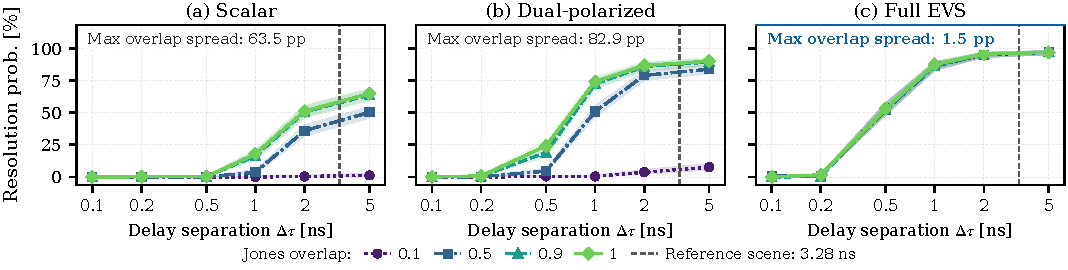
\includegraphics[width=\textwidth]{fig_resolvability.pdf}
\caption{Panel separability at $-10$~dB: resolution probability against
cascaded-delay separation, one curve per Jones overlap
$|\be_k^{\mathsf H}\be_{k'}|$ of the closest-delay pair, $480$ trials per
cell with exact $95\%$ Clopper--Pearson bands.}
\label{fig:c1_separability}
\end{figure*}

\begin{figure*}[!tb]
\centering
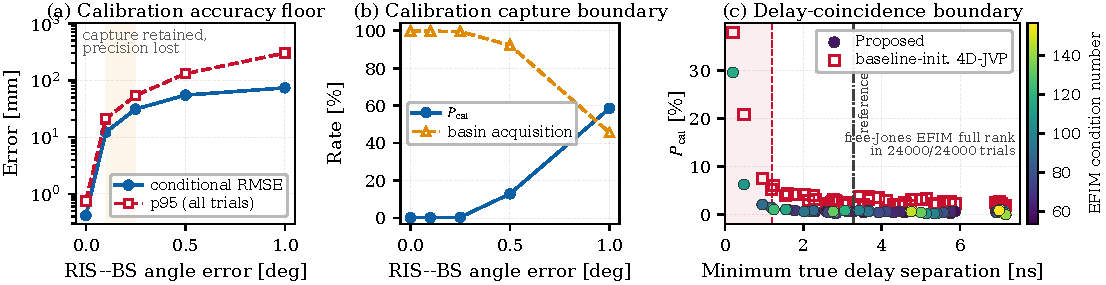
\includegraphics[width=\textwidth]{fig_boundaries.pdf}
\caption{Operating boundaries at $-10$~dB, $480$ trials per cell: (a)~conditional
position RMSE and all-trial 95th percentile (p95) versus RIS--BS angle error; (b)~position
catastrophic and basin-acquisition rates; and (c)~position catastrophic rate
versus the minimum cascaded-delay separation. In~(c), the shaded strip is the
delay-coincidence region, color denotes the median free-Jones EFIM condition
number, and thin segments connect the proposed and baseline-initialized
4D-JVP routes at the same position rather
than fitting a trend.}
\label{fig:boundaries}
\end{figure*}

\subsection{Robustness and Deployment Limits}
\label{subsec:res_robustness}
Among the tested ranges, RIS--BS calibration
is the most restrictive (Fig.~\ref{fig:boundaries}(a)--(b)): angular error
degrades precision before it degrades acquisition reliability, raising
conditional RMSE from $0.416$
to $31.1$~mm at $0.25^\circ$ even though the basin-acquisition rate remains
$99.58\%$; at $1^\circ$, the position catastrophic rate reaches $58.54\%$.

In the dedicated $0$-dB model-order sweep, underestimating $K$ with
$\widehat K=2$ gives a $0.705$-m median and
$P_{\rm cat}=65.6\%$; overestimating it with $\widehat K=4$ or $5$ preserves
submillimeter medians but yields position catastrophic rates above one third.

Delay coincidence limits acquisition even where the local EFIM remains
nonsingular (Fig.~\ref{fig:boundaries}(c)). Across a $5\times5\times2$
position grid, the proposed median per-position catastrophic rate is $0.62\%$
against $2.71\%$ for baseline-initialized 4D-JVP\@. The two worst grid corners
lie near a cascaded-delay coincidence surface; the worst reaches $29.58\%$ at
a minimum separation of $0.062/B_{\rm occ}$ ($0.197$~ns), while the free-Jones
EFIM remains full rank at every tested position, including those corners.
Deployment screening should include a delay-coincidence check and a coarse
global fallback in addition to a PEB map.

A $25\%$ cyclic prefix at $\Delta f=5$~MHz lasts $50$~ns and covers the $19.1$-ns delay span
over the clock-search interval. With one configuration per $250$-ns OFDM
symbol, $T=256$ configurations span about $64$~\textmu s, the block-static interval
required by (A6).
\section{Conclusion}
\label{sec:conclusion}

Receiver-mode selection and cascaded-delay coincidence expose acquisition
risks that the free-Jones EFIM does not exclude. A reduced receiver can make
a panel pair difficult to resolve even when a single-panel free-Jones EFIM remains
finite. At the worst tested position-grid point, the multi-panel EFIM is full
rank but the position catastrophic rate is $29.58\%$. Deployment checks
need receiver-separability and delay-coincidence assessments alongside a PEB
map.

MKSC-GI projects out noise-only receive directions before delay acquisition
and fits a common panel geometry. CCOP-JVP profiles the clock at fixed
position and uses a deterministic objective-gap certificate for its inner
solution. In
the controlled Phase-II comparison, it matches the explicit-clock route's
RMSE while reducing the outer dimension from four to three. For the
calibrated reference scene with known $K$ and the matched center-frequency
spatial model, the $-10$-dB end-to-end median position error is $0.32$~mm;
position and clock catastrophic rates are $0.42\%$ and $0.31\%$. Scaling to
larger panel counts calls for association without factorial permutation
search.

\IEEEtriggeratref{17}
\bibliographystyle{IEEEtran}
\bibliography{references}

\end{document}
